\documentclass[11pt,a4paper,oneside]{report}

% ---------------------------------------------------------------------------
% EDIT THESE FIELDS ONCE; THEY are reused throughout the report.
% ---------------------------------------------------------------------------
\newcommand{\studentname}{Aryan Satyendra Kumar}
\newcommand{\studentid}{[Student ID]}
\newcommand{\degreeprogramme}{[Degree Programme]}
\newcommand{\institution}{[Institution / University]}
\newcommand{\hostorganisation}{[Host Organisation / Laboratory]}
\newcommand{\academicsupervisor}{[Academic Supervisor]}
\newcommand{\industrysupervisor}{[Internship Supervisor]}
\newcommand{\internshipperiod}{June--July 2026}
\newcommand{\submissiondate}{July 2026}
\newcommand{\projecttitle}{Multimodal Roadside PM$_{2.5}$ Prediction Using Visual, Geospatial, Sensor and Atmospheric Context}

\usepackage[T1]{fontenc}
\usepackage[utf8]{inputenc}
\usepackage{lmodern}
\usepackage{microtype}
\usepackage[a4paper,top=24mm,bottom=25mm,left=27mm,right=24mm,headheight=15pt]{geometry}
\usepackage{graphicx}
\usepackage{booktabs}
\usepackage{longtable}
\usepackage{tabularx}
\usepackage{array}
\usepackage{multirow}
\usepackage{adjustbox}
\usepackage{amsmath,amssymb}
\usepackage{siunitx}
\usepackage[dvipsnames,table]{xcolor}
\usepackage{enumitem}
\usepackage{caption}
\usepackage{subcaption}
\usepackage{float}
\usepackage{fancyhdr}
\usepackage{titlesec}
\usepackage{url}
\usepackage{hyperref}
\usepackage{bookmark}

\definecolor{Navy}{HTML}{102A56}
\definecolor{Blue}{HTML}{2F66B0}
\definecolor{Teal}{HTML}{1597A5}
\definecolor{Green}{HTML}{2E7D32}
\definecolor{Orange}{HTML}{E67E22}
\definecolor{Red}{HTML}{C0392B}
\definecolor{Purple}{HTML}{6C4AB6}
\definecolor{LightBlue}{HTML}{ECF3FF}
\definecolor{LightGray}{HTML}{F4F7FB}

\hypersetup{
  colorlinks=true,
  linkcolor=Navy,
  citecolor=Green,
  urlcolor=Blue,
  pdftitle={\projecttitle},
  pdfauthor={\studentname}
}
\graphicspath{{figures/}}
\captionsetup{font=small,labelfont=bf}
\setlist[itemize]{leftmargin=*,itemsep=3pt,topsep=4pt}
\setlist[enumerate]{leftmargin=*,itemsep=3pt,topsep=4pt}
\setlength{\parindent}{0pt}
\setlength{\parskip}{5.5pt}
\setlength{\emergencystretch}{3em}
\renewcommand{\arraystretch}{1.16}
\sisetup{detect-all,group-separator={,},group-minimum-digits=4}

\pagestyle{fancy}
\fancyhf{}
\fancyhead[L]{\small\color{Navy}Roadside PM Visual Intelligence}
\fancyhead[R]{\small\color{Navy}\leftmark}
\fancyfoot[C]{\thepage}
\renewcommand{\headrulewidth}{0.4pt}

\titleformat{\chapter}[display]
  {\normalfont\bfseries\color{Navy}}
  {\filleft\Large\chaptertitlename\ \thechapter}
  {4pt}
  {\titlerule\vspace{7pt}\Huge}
  [\vspace{5pt}\titlerule]
\titleformat{\section}{\Large\bfseries\color{Navy}}{\thesection}{0.7em}{}
\titleformat{\subsection}{\large\bfseries\color{Blue}}{\thesubsection}{0.7em}{}

\newcommand{\pmtwo}{PM$_{2.5}$}
\newcommand{\ugm}{\si{\micro\gram\per\cubic\metre}}
\newcommand{\Rtwo}{$R^2$}
\newcommand{\cautionbox}[1]{%
  \begin{center}
  \fcolorbox{Red}{red!5}{\parbox{0.91\textwidth}{\textbf{\color{Red}Scientific caution.} #1}}
  \end{center}}
\newcommand{\resultbox}[1]{%
  \begin{center}
  \fcolorbox{Green}{green!5}{\parbox{0.91\textwidth}{\textbf{\color{Green}Result.} #1}}
  \end{center}}

\begin{document}

\begin{titlepage}
  \centering
  \vspace*{16mm}
  {\Large\bfseries\color{Navy}INTERNSHIP PROJECT REPORT\par}
  \vspace{13mm}
  {\Huge\bfseries\color{Navy}\projecttitle\par}
  \vspace{7mm}
  {\Large Roadside PM Visual Intelligence\par}
  \vspace{16mm}
  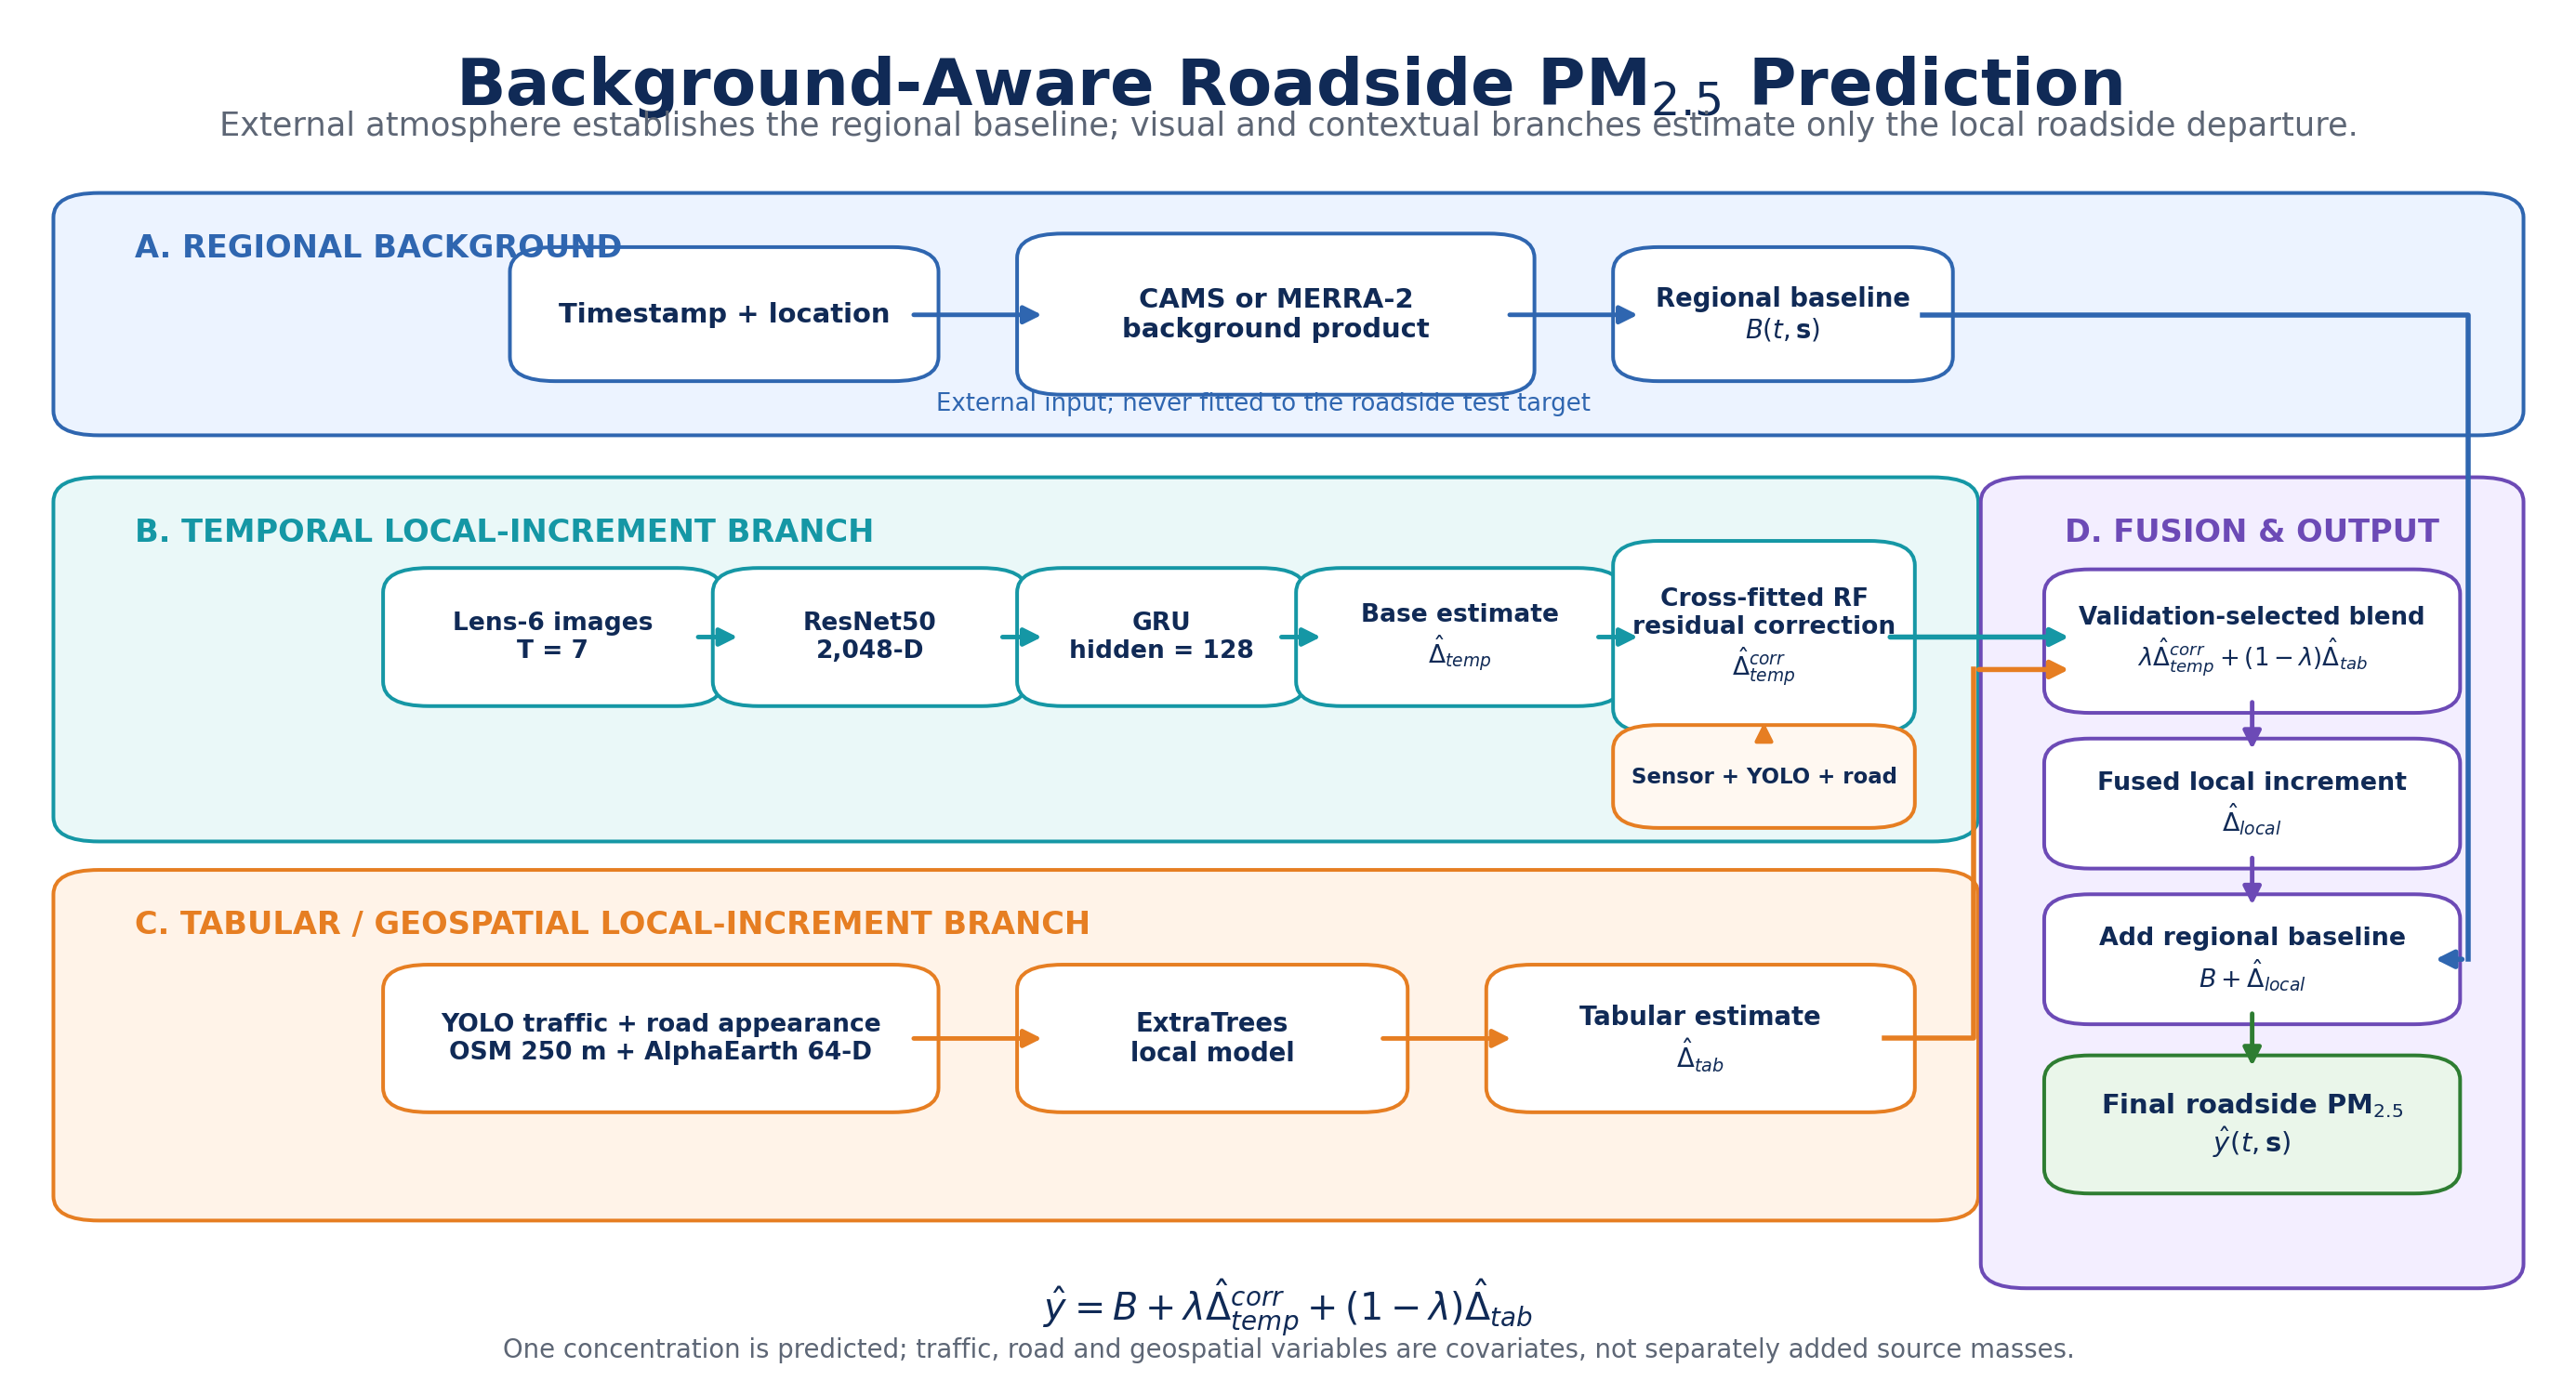
\includegraphics[width=0.92\textwidth]{current_architecture.png}
  \vfill
  \begin{tabular}{rl}
    \textbf{Submitted by:} & \studentname\ (\studentid)\\
    \textbf{Programme:} & \degreeprogramme\\
    \textbf{Institution:} & \institution\\
    \textbf{Host:} & \hostorganisation\\
    \textbf{Academic supervisor:} & \academicsupervisor\\
    \textbf{Internship supervisor:} & \industrysupervisor\\
    \textbf{Internship period:} & \internshipperiod\\
    \textbf{Report date:} & \submissiondate
  \end{tabular}
  \vspace{12mm}
\end{titlepage}

\pagenumbering{roman}

\chapter*{Declaration}
\addcontentsline{toc}{chapter}{Declaration}
I declare that this report is an accurate account of the engineering and research work
performed in the \emph{Roadside PM Visual Intelligence} codebase during the stated
internship period. Results are reported with their validation protocol and known
limitations. High random-window scores are explicitly separated from whole-date
generalisation tests. External atmospheric products are identified as model or
reanalysis estimates rather than roadside reference measurements. The source
attribution experiments are described as exploratory particle or source proxies and
are not presented as validated chemical apportionment.

\vspace{18mm}
\begin{tabularx}{\textwidth}{X X}
  \textbf{Student signature:} \hrulefill & \textbf{Date:} \hrulefill
\end{tabularx}

\chapter*{Acknowledgements}
\addcontentsline{toc}{chapter}{Acknowledgements}
I thank my supervisors, the data collection team and the contributors to the
TRAQID and MUMMA datasets for making this work possible. I also acknowledge the
open-source communities behind PyTorch, scikit-learn, OpenStreetMap, Ultralytics,
Hugging Face, Copernicus CAMS, NASA MERRA-2 and the geospatial data services used
in this project. The editable supervisor and organisation fields on the title page
should be completed before formal submission.

\chapter*{Abstract}
\addcontentsline{toc}{chapter}{Abstract}
This internship developed and audited a reproducible multimodal system for predicting
roadside \pmtwo\ from a moving platform. The project began with a high-scoring
image-sequence model on the historical TRAQID dataset and evolved into a more
scientifically defensible five-day MUMMA study. The final data pipeline aligned
\num{6873} ten-second sensor observations from 55 runs with \num{20619}
preprocessed images from three camera lenses. It extracted 58 YOLO traffic
features, 45 road-appearance features, 25 OpenStreetMap context features, 64
AlphaEarth embedding dimensions and 24 non-PM sensor, meteorology, time and
mobility variables. External CAMS and MERRA-2 atmospheric products were added to
separate regional background pollution from the local roadside increment.

The work compared direct tabular regression, frozen-CNN embeddings, GRU and LSTM
sequence models, residual correction, background-plus-local-increment models,
nested temporal-tabular ensembles, feature selection and early image-atmosphere
fusion. A central finding was that random splitting of overlapping T=7 sequences
produced optimistic scores: 98.32\% of five-day test targets had already appeared
as training context. Under whole-date holdout, direct image models generalised
poorly. CAMS background decomposition improved the pooled five-day result to
\Rtwo\ approximately 0.46. Replacing CAMS with MERRA-2 further improved the
validation-selected nested ensemble to MAE 22.58 \ugm, RMSE 35.69 \ugm\ and pooled
\Rtwo\ 0.538. A fixed 50:50 ensemble reached pooled \Rtwo\ 0.566 but was retained
only as a diagnostic because its weight was not validation-selected. Mean per-date
\Rtwo\ remained negative, showing that new-day stability is not yet established.

The internship also explored particle-size regimes, NMF source-proxy components,
assumption-conditioned source scenarios, spatial variograms, feature relevance,
extreme-event audits and conformal uncertainty. These analyses established clear
limits: chemical source apportionment requires differential OPC bins and chemical
reference evidence, while future deployment claims require a frozen model evaluated
once on untouched dates. The principal outcome is therefore both an improved model
and a rigorous validation framework that distinguishes diagnostic accuracy from
real generalisation.

\tableofcontents
\listoffigures
\listoftables
\clearpage
\pagenumbering{arabic}

\chapter{Introduction}

\section{Motivation}
Roadside \pmtwo\ varies over multiple spatial and temporal scales. A moving sensor
observes the sum of a broad atmospheric background, neighbourhood-scale land-use
effects and short-lived local increments from traffic, resuspension, road activity
and meteorological mixing. A camera can observe traffic and road context, but it
cannot directly measure aerosol mass. Conversely, a regional atmospheric product
can describe the broad pollution regime but cannot resolve the exact plume or
street-level exposure beside a moving vehicle. The project therefore treated
roadside prediction as a multimodal inference problem rather than a pure
image-regression task.

The work also confronted a validation problem. Consecutive frames sampled every ten
seconds are strongly autocorrelated. A T=7 sliding window shares six frames with the
next window. If windows are constructed first and then randomly shuffled, nearly
identical context enters both training and test partitions. The resulting score may
be useful as a software or same-distribution diagnostic, but it is not evidence that
the model will generalise to a new date. Resolving this distinction became a major
scientific contribution of the internship.

\section{Project objectives}
The project had five linked objectives:
\begin{enumerate}
  \item build a reproducible pipeline from raw sensor files and multi-lens videos
        to aligned modelling records;
  \item derive interpretable traffic, road, sensor, geospatial and atmospheric
        predictors without using PM or OPC target proxies as reportable inputs;
  \item compare image-only, tabular, temporal, residual and background-decomposition
        architectures;
  \item establish leakage audits and whole-date evaluation as the principal
        generalisation test; and
  \item explore particle-size and source-proxy analyses while preserving the
        distinction between predictive association and chemical source
        apportionment.
\end{enumerate}

\section{Main contributions}
The internship produced the following concrete outputs:
\begin{itemize}
  \item a five-day canonical MUMMA table with \num{6873} aligned observations;
  \item \num{20619} preprocessed images and a manifest enforcing exactly one image
        per retained lens and sample;
  \item complete YOLO traffic, road segmentation, OSM, AlphaEarth and atmospheric
        feature pipelines;
  \item reusable frozen-CNN, GRU/LSTM, classical regression, residual correction
        and nested ensemble implementations;
  \item explicit overlap audits for random temporal splits;
  \item whole-date and nested validation protocols;
  \item a MERRA-2 background-plus-local-increment candidate with pooled whole-date
        \Rtwo\ 0.538 under validation-selected fusion;
  \item uncertainty, feature relevance, variogram and sudden-event diagnostics;
        and
  \item consolidated experiment and architecture registries for reproducibility.
\end{itemize}

\begin{figure}[H]
  \centering
  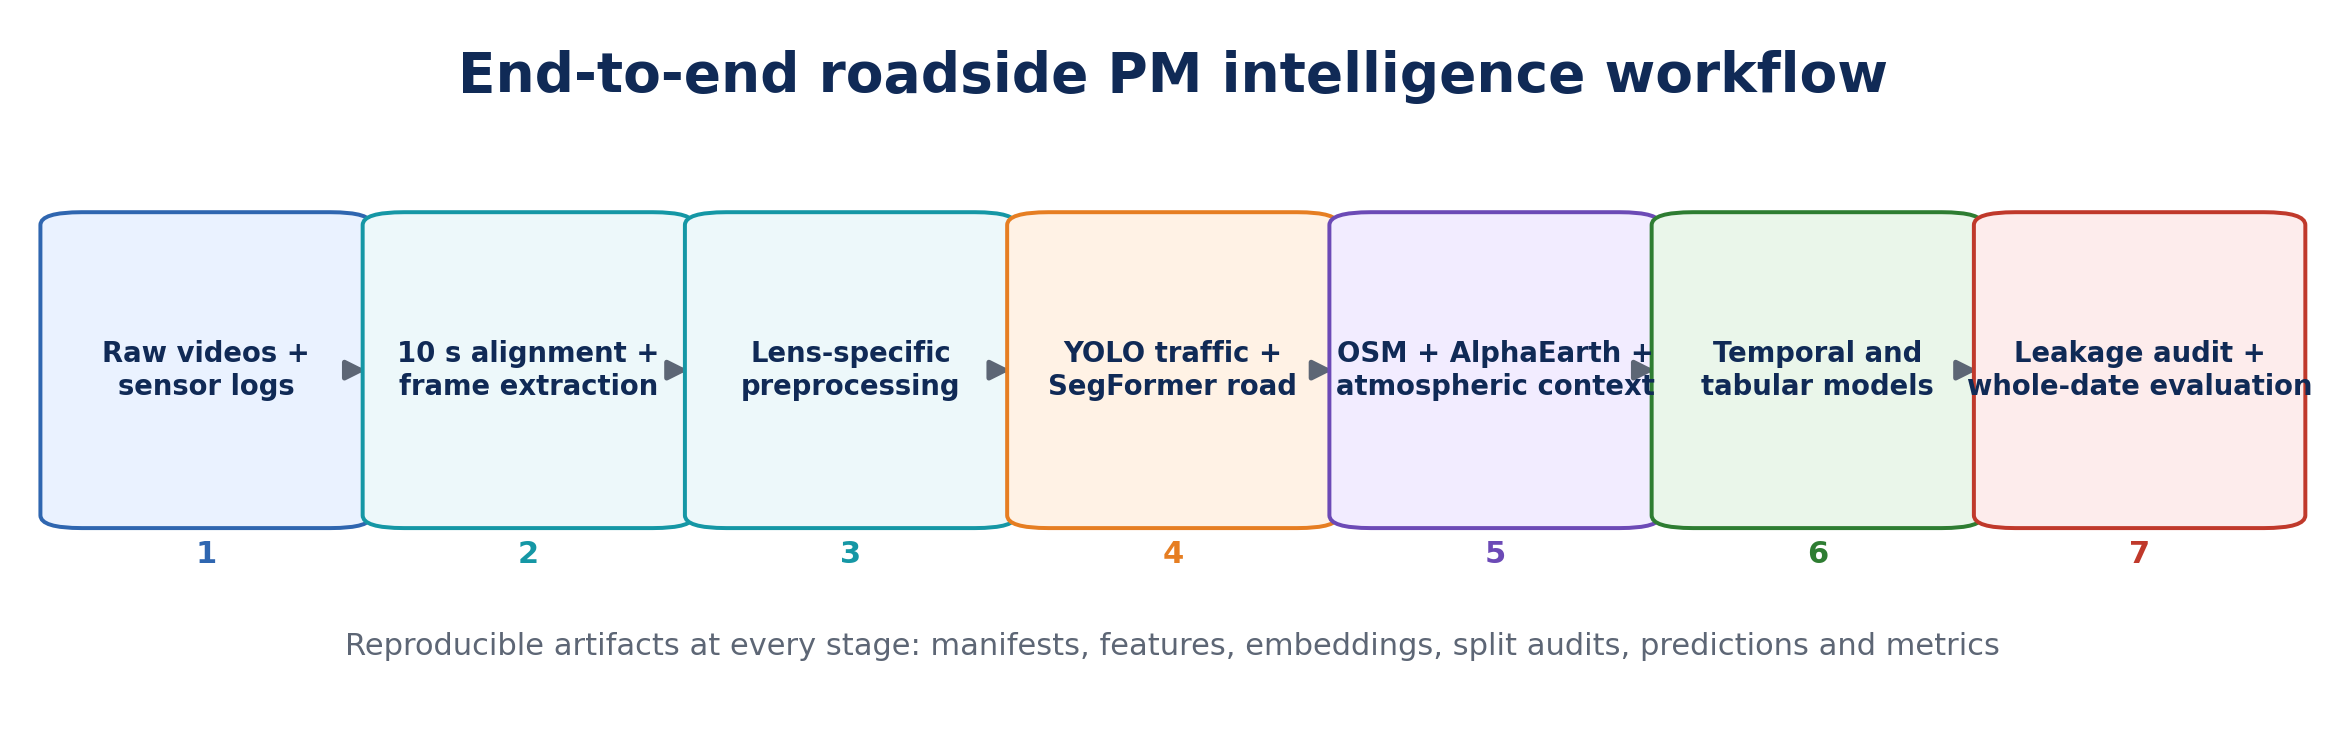
\includegraphics[width=\textwidth]{project_pipeline.png}
  \caption{End-to-end workflow developed during the internship. Each stage writes
  a manifest, feature table, model artifact or audit file so that downstream
  results can be traced to their source.}
  \label{fig:pipeline}
\end{figure}

\section{Report scope and terminology}
This report covers the historical TRAQID reproduction, the initial two-day MUMMA
pilot, the complete five-day MUMMA experiments, the newer CAMS and MERRA-2
background studies, architecture-2 early fusion, uncertainty and exploratory
particle/source work. In this report:
\begin{itemize}
  \item \emph{random diagnostic} means a split in which neighbouring rows or
        overlapping sequences can occur in different partitions;
  \item \emph{fair} means that complete dates are withheld from model fitting;
  \item \emph{pooled \Rtwo} is computed after concatenating predictions from all
        held-out dates;
  \item \emph{mean fold \Rtwo} is the arithmetic mean of the five date-specific
        \Rtwo\ values; and
  \item \emph{source proxy} denotes a latent or assumption-conditioned component,
        not a chemically validated source contribution.
\end{itemize}

\chapter{Scientific and Technical Background}

\section{A scale-decomposition view of roadside \pmtwo}
The final architecture is motivated by a simple mass-concentration decomposition:
\begin{equation}
  y(t,\mathbf{s}) = B(t,\mathbf{s}) + \Delta_{\mathrm{local}}(t,\mathbf{s}) + \epsilon,
  \label{eq:decomposition}
\end{equation}
where $y$ is the roadside sensor concentration, $B$ is the broad atmospheric
background, $\Delta_{\mathrm{local}}$ is the local departure from that background
and $\epsilon$ includes instrument noise, alignment error and unmodelled processes.
The terms are not separate physical samples collected by this project. They are a
modelling decomposition. The external product supplies $B$; the machine-learning
branches estimate $\Delta_{\mathrm{local}}$ from non-PM predictors.

This decomposition explains why traffic, road and land-use features remain useful
even when images and atmospheric products are present. The atmospheric product is
too coarse to resolve near-road variability. A generic image embedding contains
visual appearance but does not explicitly guarantee stable vehicle counts, road
texture or land-use context. Engineered variables expose these factors to a
low-data tabular model and make the correction more auditable. They are predictive
covariates, not separate mass contributions that are arithmetically added.

\section{CAMS, MERRA-2 and local observations}
The Copernicus Atmosphere Monitoring Service (CAMS) combines atmospheric modelling,
emissions, meteorology and data assimilation to provide gridded aerosol and gas
fields. MERRA-2 is a NASA atmospheric reanalysis that assimilates observations into
a global numerical model and provides aerosol species and meteorological context.
Neither product is a roadside reference monitor, and neither simply assigns a
satellite pixel's PM value to an image. They provide a regional estimate for a grid
cell and time. The project aligned these external estimates to each roadside sample
by timestamp and representative location.

In the earlier CAMS implementation, a small number of distinct time-grid values were
repeated across many ten-second rows because the drive occupied a small region
relative to the atmospheric grid and CAMS changed at a much coarser time step.
MERRA-2 supplied more distinct matched atmospheric records and, in this dataset,
proved a stronger baseline for the local-increment model. The background is
available at inference time and must therefore also be supplied for an unseen date;
it is not merely a training or tuning variable.

\section{Images, CNN embeddings and temporal models}
A convolutional neural network maps each frame to a feature vector encoding visual
patterns. Frozen ImageNet backbones were used to reduce overfitting in the small
five-day dataset. ResNet50 produced a 2,048-dimensional global-average-pooled
embedding. ConvNeXt-tiny, MobileNetV2, EfficientNet-B0 and VGG16 representations
were also supported or tested.

A recurrent neural network receives a sequence of embeddings
$\mathbf{x}_{t-T+1},\ldots,\mathbf{x}_{t}$ and produces a temporal representation:
\begin{equation}
  \mathbf{h}_t = \mathrm{GRU}(\mathbf{x}_{t-T+1:t}), \qquad
  \hat y_t = g(\mathbf{h}_t).
\end{equation}
GRUs and LSTMs can capture persistence and evolving visual context. However, the
same persistence makes random splitting dangerous: overlapping windows can share
raw frames across partitions.

\section{Tree ensembles and residual learning}
Random Forest averages decorrelated decision trees trained on bootstrap samples.
ExtraTrees further randomises split thresholds, often producing a strong nonlinear
model for mixed tabular variables. HistGradientBoosting adds shallow trees
sequentially to reduce residual error. Ridge provides a regularised linear
reference.

Residual learning begins with a base prediction $\hat y_{\mathrm{base}}$ and fits a
second model to
\begin{equation}
  r = y-\hat y_{\mathrm{base}}.
\end{equation}
The corrected prediction is $\hat y=\hat y_{\mathrm{base}}+\hat r$. To prevent
the residual model from learning errors caused by in-sample base predictions, the
project used out-of-fold or cross-fitted base predictions wherever possible.

\section{Evaluation metrics}
The report uses:
\begin{align}
  \mathrm{MAE} &= \frac{1}{n}\sum_i |y_i-\hat y_i|,\\
  \mathrm{RMSE} &= \sqrt{\frac{1}{n}\sum_i(y_i-\hat y_i)^2},\\
  R^2 &= 1-\frac{\sum_i(y_i-\hat y_i)^2}{\sum_i(y_i-\bar y)^2}.
\end{align}
MAE measures typical absolute error; RMSE penalises extreme misses more strongly.
\Rtwo\ compares squared error with a mean-prediction baseline. A negative
date-specific \Rtwo\ means the model was worse on that date than predicting that
date's mean. Pooled \Rtwo\ can still be positive if the model captures differences
between daily means, even when within-day fluctuations remain difficult.

\chapter{Datasets and Data Engineering}

\section{TRAQID historical benchmark}
The historical benchmark contained \num{26558} T=7 front/rear image sequences.
The presentation reproduction randomly assigned \num{21246} sequences to
training/validation and \num{5312} to test. Because overlapping windows were
shuffled, the experiment reproduced a high same-distribution score but was not a
future-date evaluation. TRAQID remained valuable for verifying architecture code,
residual learning and later CAMS/MERRA comparisons.

\section{MUMMA two-day pilot}
The initial pilot used 2,167 aligned records from 1 and 3 February 2026. It
established:
\begin{itemize}
  \item SSD ingestion without modifying the raw external data;
  \item ten-second sensor aggregation;
  \item multi-lens video discovery and timestamp alignment;
  \item frame extraction and lens-specific orientation/cropping;
  \item YOLO, road, CNN embedding and sequence generation;
  \item direct and residual modelling; and
  \item the first explicit overlap audit.
\end{itemize}
Lenses 1, 2 and 6 were retained after inspecting orientation and usable road
context.

\section{Canonical five-day MUMMA dataset}
The complete dataset covers 1--5 February 2026. It contains \num{6873} aligned
ten-second samples from 55 runs and exactly three preprocessed frames per sample.
Table~\ref{tab:dailycoverage} summarises the data.

\begin{table}[H]
  \centering
  \caption{Five-day MUMMA coverage. Time bounds include gaps between separate
  runs and should not be interpreted as continuous driving duration.}
  \label{tab:dailycoverage}
  \begin{tabular}{lrrrr}
    \toprule
    Date & Rows & Runs & First timestamp & Last timestamp\\
    \midrule
    2026-02-01 & 1,265 & 10 & 08:27:06 & 14:57:47\\
    2026-02-02 & 1,736 & 15 & 09:12:52 & 17:15:34\\
    2026-02-03 &   902 &  4 & 10:58:02 & 14:51:19\\
    2026-02-04 & 1,542 & 16 & 08:58:49 & 14:06:01\\
    2026-02-05 & 1,428 & 10 & 08:33:40 & 13:31:57\\
    \midrule
    Total & 6,873 & 55 & \multicolumn{2}{c}{Five collection dates}\\
    \bottomrule
  \end{tabular}
\end{table}

\begin{figure}[H]
  \centering
  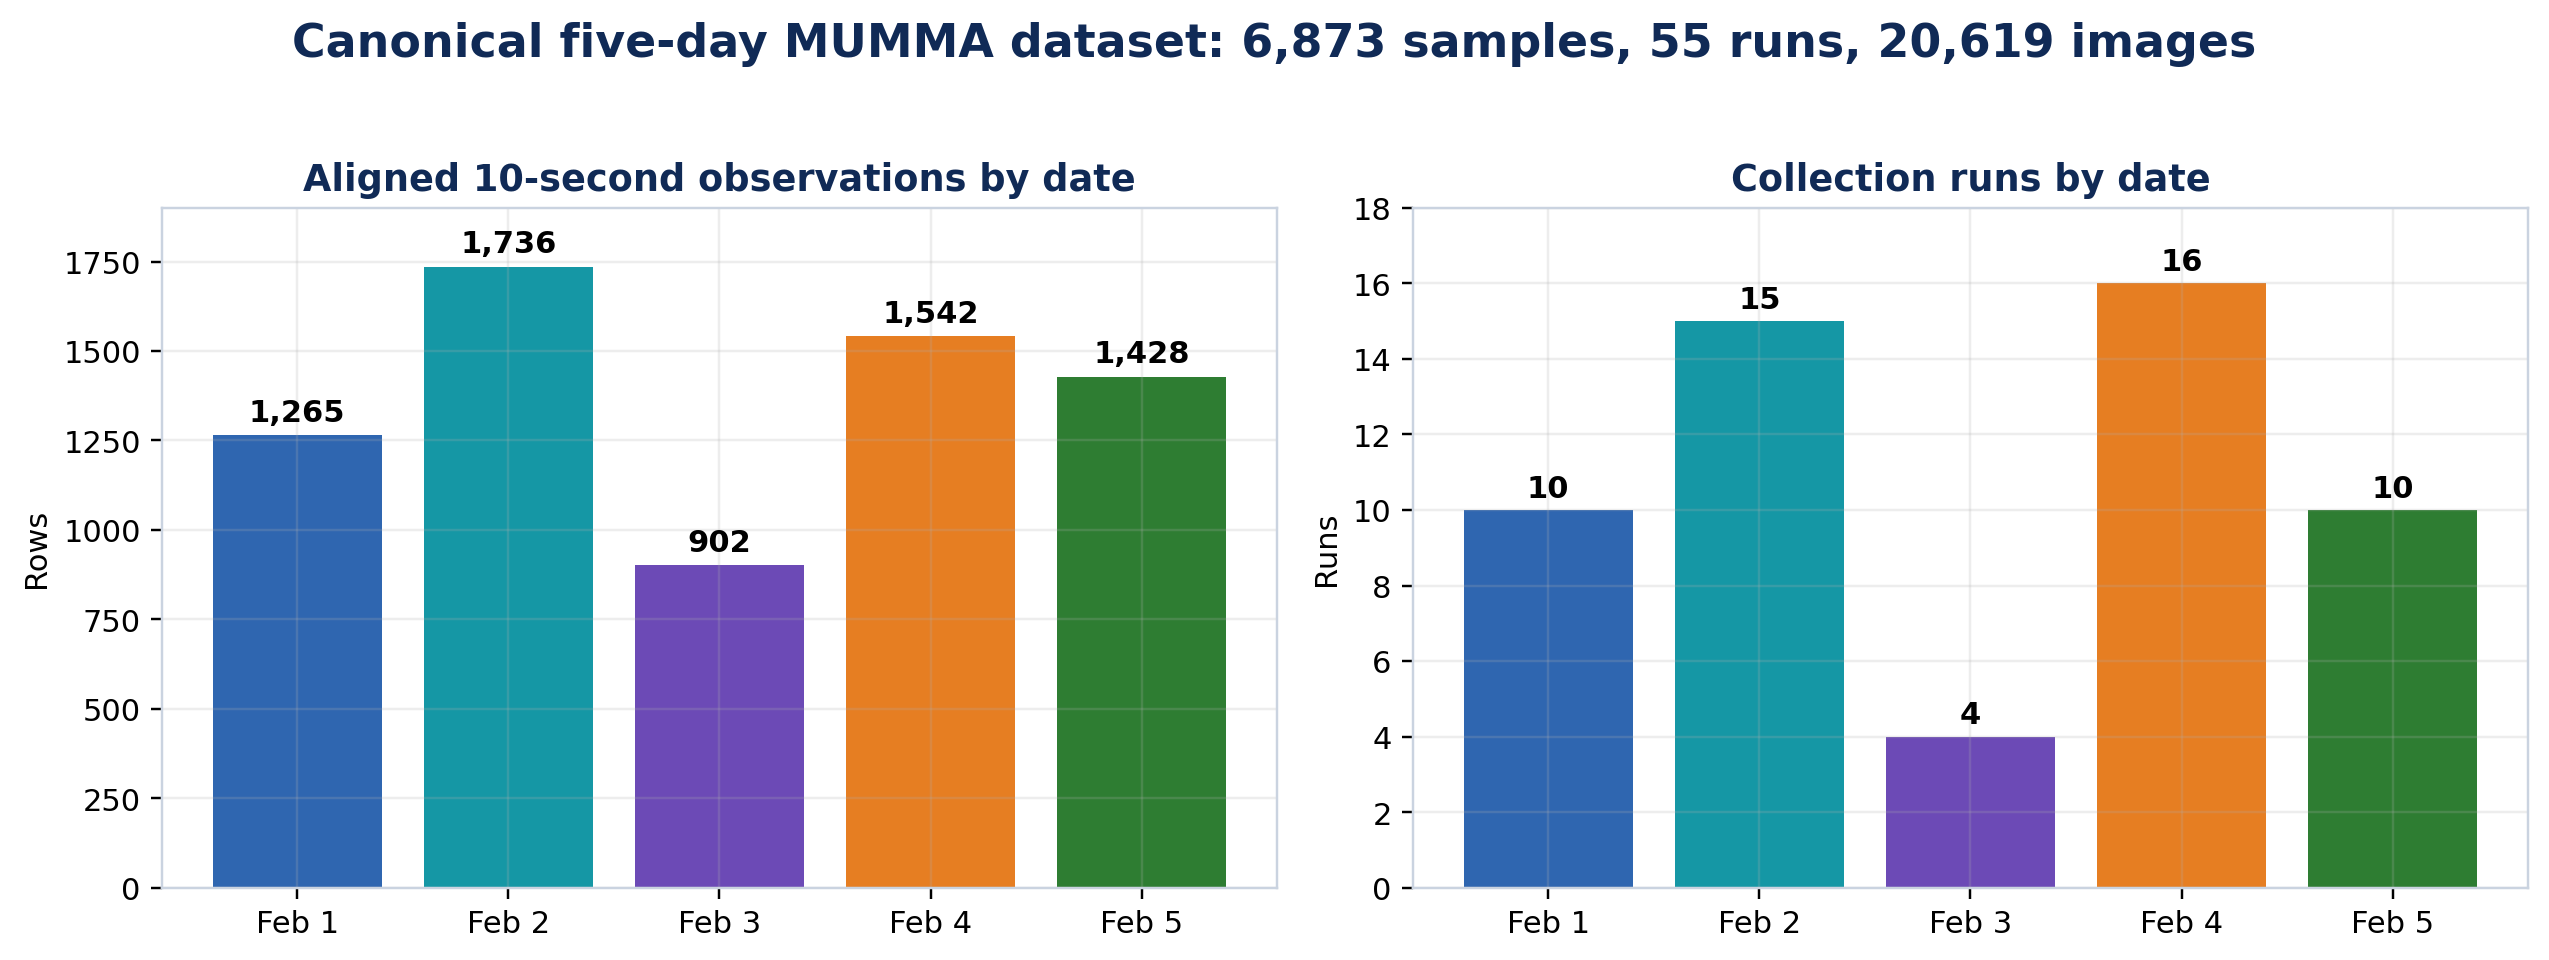
\includegraphics[width=0.92\textwidth]{mumma_dataset_summary.png}
  \caption{Distribution of aligned observations and collection runs across the
  five dates.}
  \label{fig:dataset}
\end{figure}

\section{Alignment and identity policy}
The canonical merge enforced a strict identity policy:
\begin{enumerate}
  \item \texttt{sample\_id} is unique at the sensor-record level;
  \item each sample has exactly one successful frame for lenses 1, 2 and 6;
  \item sequences are grouped by \texttt{run\_id};
  \item fair sequences cannot cross a run or date boundary; and
  \item all feature tables join through explicit sample identifiers rather than
        row position.
\end{enumerate}
The combined manifest contained \num{20619} frame rows, all successfully
preprocessed. The raw SSD remained unchanged; processed outputs were written to
the project artifact tree.

\begin{figure}[H]
  \centering
  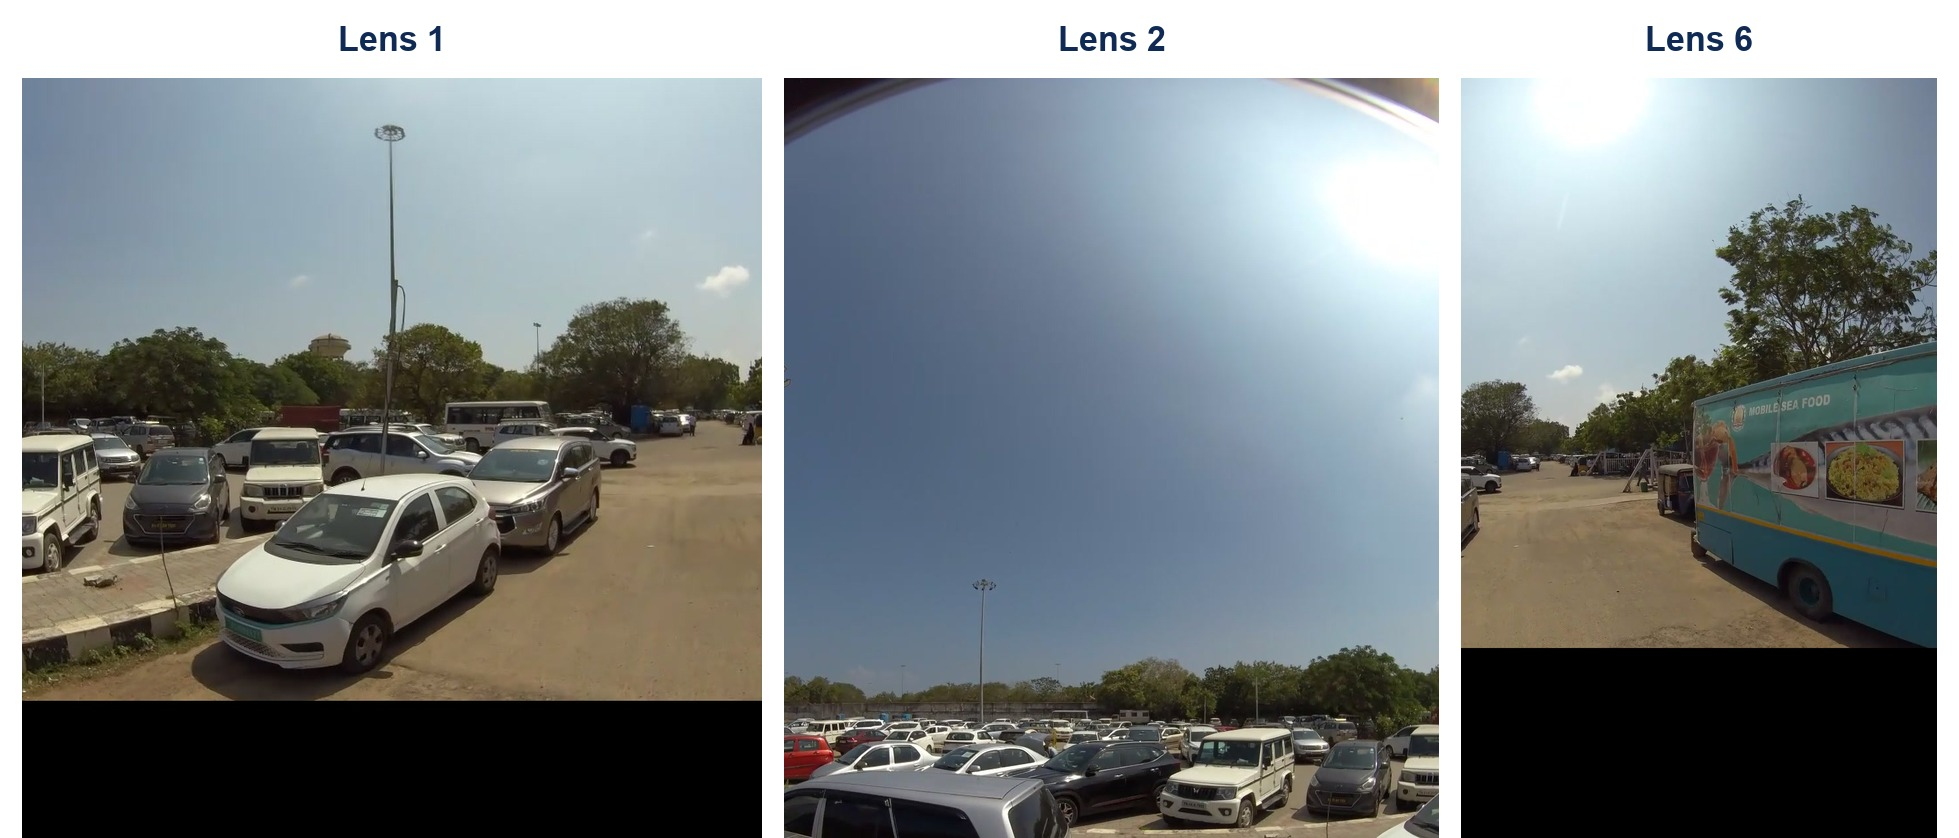
\includegraphics[width=0.96\textwidth]{mumma_multiview_sample.jpg}
  \caption{Example of the three retained preprocessed camera views for one
  aligned sample. Different views provide complementary road, sky and traffic
  context; they are not assumed to be interchangeable.}
  \label{fig:multiview}
\end{figure}

\section{Target and predictor safety}
The primary target was the sensor field \texttt{sPM2}. The reportable predictor
groups exclude \texttt{sPM1}, \texttt{sPM2}, \texttt{sPM4}, \texttt{sPM10},
OPC number channels and \texttt{sTPS}. These channels were retained only for
target construction, quality checks and exploratory particle-regime analysis.
This separation prevents direct PM or near-equivalent OPC leakage into the
roadside \pmtwo\ predictor.

\chapter{Feature Engineering}

\section{Feature-family overview}
The authoritative feature membership is stored in
\path{artifacts/runs/mumma_5day_complete_nonpm_models_v1/feature_groups.json}.
Table~\ref{tab:families} summarises the principal families. Features were
generated once and then reused across model comparisons to avoid silent changes
between experiments.

\begin{table}[H]
  \centering
  \caption{Canonical non-PM feature families.}
  \label{tab:families}
  \begin{tabularx}{\textwidth}{l r X}
    \toprule
    Family & Count & Content\\
    \midrule
    Sensor/met/gas/time/mobility & 24 &
      Temperature, relative humidity, CO$_2$, VOC/NOx indices, gases,
      cyclic time, GPS, speed, course and HDOP.\\
    YOLO traffic & 58 &
      Vehicle class counts, heavy/motor totals, confidence and box geometry,
      occupancy, exhaust/resuspension proxies and per-lens variants.\\
    Road appearance & 45 &
      SegFormer road area, colour, illumination, edge, texture and haze
      descriptors, aggregated and per road-facing lens.\\
    Road depth/metric area & 16 &
      Depth percentiles, mask-cleaning diagnostics and estimated road area;
      provisional.\\
    OSM & 25 &
      Activity/POI counts and road-network hierarchy within 250 m.\\
    AlphaEarth & 64 &
      Annual latent embedding dimensions A00--A63.\\
    \bottomrule
  \end{tabularx}
\end{table}

\section{Sensor, meteorology, gases, time and mobility}
The 24 variables were:
\begin{quote}\scriptsize\raggedright
\texttt{temp}, \texttt{rh}, \texttt{k30Co2}, \texttt{sTemp},
\texttt{sRh}, \texttt{sVocI}, \texttt{sNoxI}, \texttt{co\_ppb},
\texttt{no2\_ppb}, \texttt{so2\_ppb}, \texttt{o3\_ppb\_compensated},
\texttt{ch4\_ratio}, \texttt{nh3\_ppm}, \texttt{hour\_sin},
\texttt{hour\_cos}, \texttt{minute\_sin}, \texttt{minute\_cos},
\texttt{lat}, \texttt{long}, \texttt{alt}, \texttt{sog\_clean},
\texttt{cog\_sin}, \texttt{cog\_cos}, \texttt{hdop}.
\end{quote}
Cyclic encoding prevents an artificial discontinuity between, for example,
23:59 and 00:00. Course was encoded with sine and cosine for the same reason.
Latitude and longitude were retained as predictive location variables but were
recognised as a potential route-memory mechanism in random splits.

\section{YOLO traffic features}
An IDD-trained YOLO11m detector was applied to all \num{20619} preprocessed
frames. The extraction completed successfully for every frame and produced
\num{136534} PM-relevant road-user detections. The object classes were mapped
to motorcycle, car, auto-rickshaw, truck, bus, bicycle and an unknown-vehicle
fallback.

\begin{figure}[H]
  \centering
  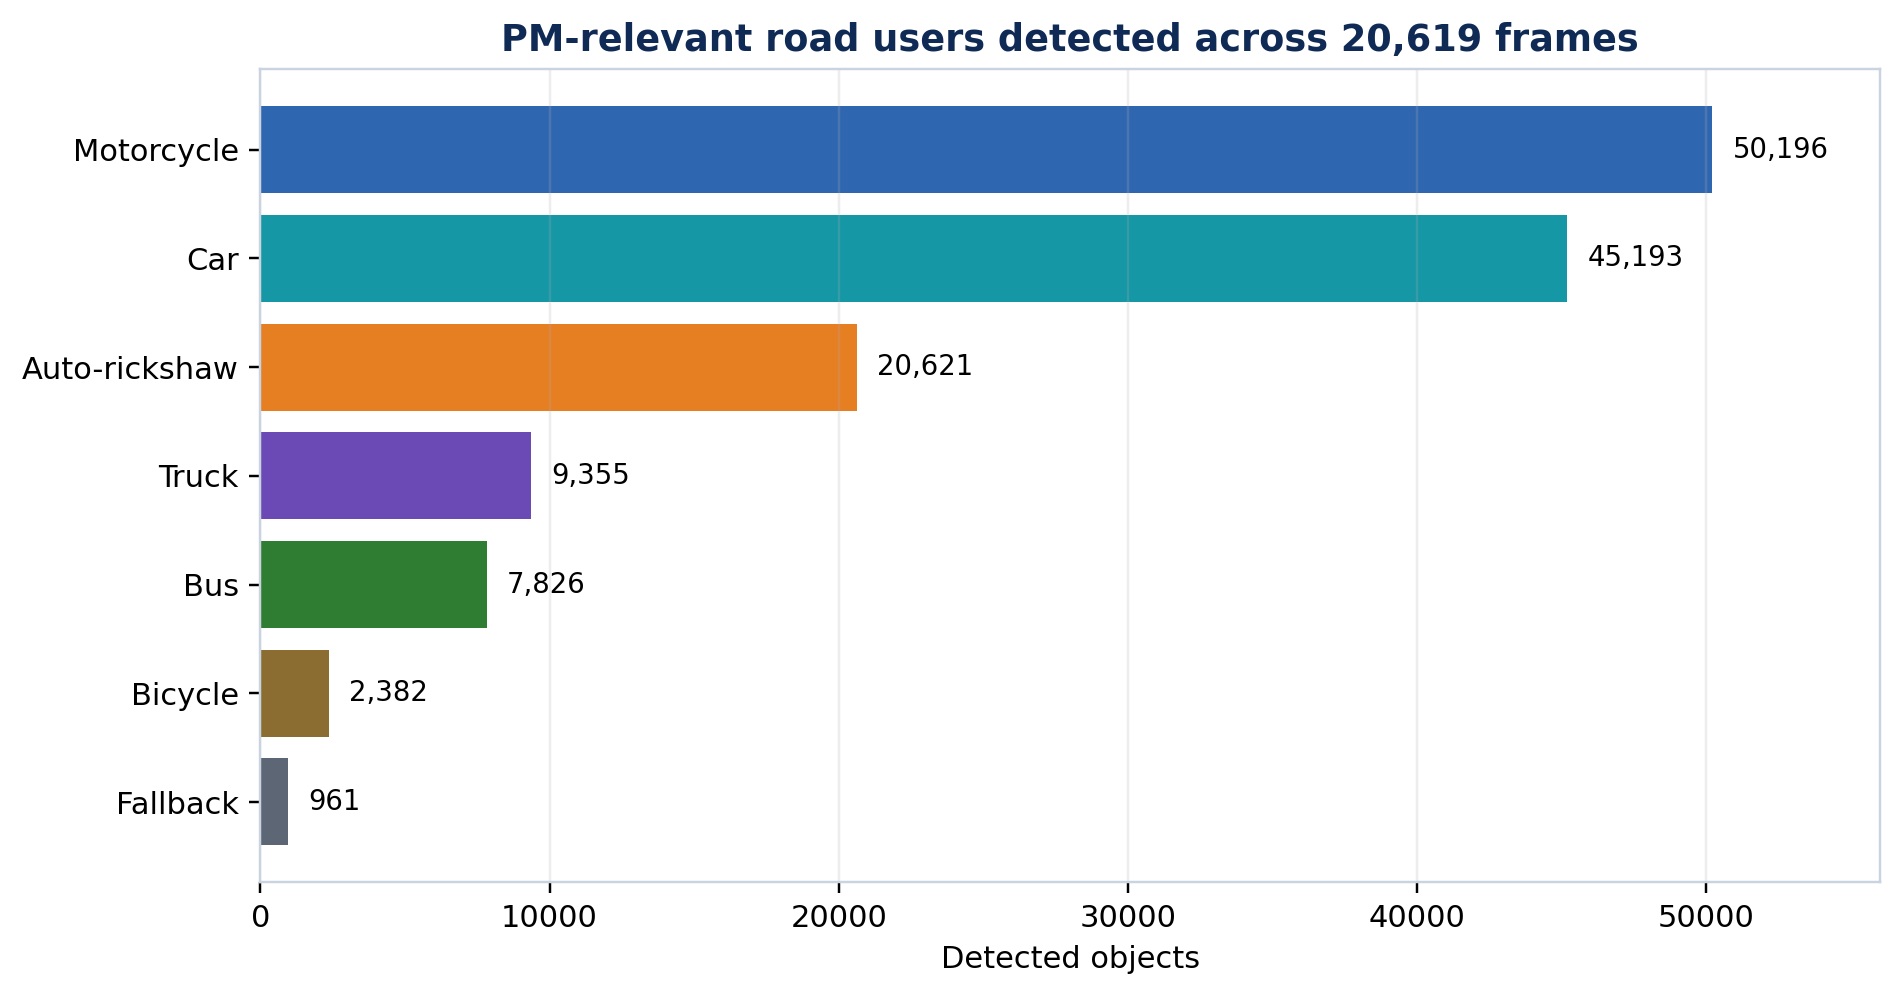
\includegraphics[width=0.86\textwidth]{yolo_object_counts.png}
  \caption{Detected PM-relevant road users in the five-day MUMMA dataset. Counts
  are observations in images, not unique physical vehicles.}
  \label{fig:yolo}
\end{figure}

The 58 model features comprise:
\begin{itemize}
  \item aggregate counts for total vehicles, heavy vehicles, motor vehicles and
        each mapped class;
  \item initial exhaust and resuspension proxy scores based on the detected mix;
  \item mean and maximum bounding-box area, average confidence and maximum
        confidence;
  \item the same core counts, proxies and geometry for lenses 1, 2 and 6; and
  \item \texttt{yolo\_lens\_count} as a view-availability audit.
\end{itemize}
These variables do not claim to measure emitted mass. They describe source
opportunity, traffic composition, proximity/occupancy and activity. A vehicle
count can correlate negatively in a global table because routes, background
pollution and time of day confound the association. Within-day centring changed
some vehicle correlations from negative to positive, demonstrating why
correlation is not a causal emission factor.

\section{Road appearance features}
A SegFormer-B0 road model was run on the calibrated road-facing lenses 1 and 6.
Of \num{13746} input frames, \num{13041} succeeded and 705 failed. The mean
segmented road-area ratio among successes was 0.1163.

Eleven underlying measurements were used:
\begin{enumerate}
  \item road area ratio;
  \item mean brightness;
  \item mean saturation;
  \item contrast standard deviation;
  \item shadow-pixel ratio;
  \item glare-pixel ratio;
  \item brown-pixel ratio;
  \item gray/dry-pixel ratio;
  \item edge density;
  \item Laplacian texture standard deviation; and
  \item haze-flatness proxy.
\end{enumerate}
Each measurement was represented as an all-lens mean, all-lens maximum, lens-1
value and lens-6 value, with an additional road-lens count. These variables
describe visible road state and surface opportunity for resuspension; they do
not measure the amount of road dust suspended in air.

\section{Depth-derived road area}
A depth-assisted procedure attempted to convert the road mask to an estimated
metric area. It produced a value for all \num{6873} samples, with mean
\SI{89.48}{\square\metre}, but every result was flagged either
\texttt{needs\_visual\_review} or \texttt{bad\_low\_road\_mask\_area}.
The cleaning stage removed a median 54.8\% of the initial mask. Models using
this family generally degraded. It is retained as a documented negative result,
not as a trusted physical road-area measurement.

\section{OpenStreetMap context}
OpenStreetMap queries were cached by corridor tile and summarised locally inside
a 250 m radius. The final run reused 41 cached tiles, fetched one remaining tile
and wrote complete features for all \num{6873} samples. The 25 predictors were:
\begin{itemize}
  \item \textbf{activity/POI counts (14):} fuel station, restaurant, bus stop,
        parking, construction, industrial, factory, warehouse, marketplace,
        park, school/college, hospital, commercial and retail;
  \item \textbf{road context (11):} road-segment count, total road length, and
        counts of motorway, trunk, primary, secondary, tertiary, residential,
        service, living-street and unclassified roads.
\end{itemize}
Rounded coordinates and OSM location keys were join metadata and were not
counted as predictors. OSM provides slowly varying context about potential
activity and road hierarchy. It cannot describe the instantaneous traffic state.

\section{AlphaEarth embeddings}
AlphaEarth supplied a 64-dimensional annual embedding for every location. The
dimensions A00--A63 encode learned geospatial context, but their individual
physical meanings are latent. They must not be renamed as specific land-cover
types without an independent interpretation study. AlphaEarth A36 was the only
dimension selected in every nested feature-selection fold, while several other
dimensions showed repeated relevance.

\section{Atmospheric background and meteorological fields}
Atmospheric experiments used matched CAMS, MERRA-2 and ERA5 fields, including
background PM estimates, aerosol components, temperature, dew point, humidity,
wind, pressure, precipitation and solar radiation where available. The current
background-plus-local architecture uses the external PM estimate as $B$ in
Equation~\ref{eq:decomposition}. Architecture 2 instead treats 22 atmospheric
fields as ordinary early-fusion predictors.

\section{Composite feature groups}
\begin{table}[H]
  \centering
  \caption{Composite feature groups used in the principal MUMMA experiments.}
  \label{tab:composites}
  \begin{tabular}{l r}
    \toprule
    Group & Predictors\\
    \midrule
    \texttt{visual\_yolo\_road} & 103\\
    \texttt{sensor\_plus\_visual} & 127\\
    \texttt{visual\_yolo\_road\_area\_depth} & 119\\
    \texttt{sensor\_plus\_visual\_area\_depth} & 143\\
    \texttt{visual\_yolo\_road\_osm} & 128\\
    \texttt{sensor\_plus\_visual\_osm} & 152\\
    \texttt{sensor\_plus\_alphaearth} & 88\\
    \texttt{visual\_yolo\_road\_alphaearth} & 167\\
    \texttt{sensor\_plus\_visual\_alphaearth} & 191\\
    \texttt{visual\_yolo\_road\_osm\_alphaearth} & 192\\
    \texttt{sensor\_plus\_visual\_osm\_alphaearth} & 216\\
    \bottomrule
  \end{tabular}
\end{table}

\chapter{Model Architectures}

\section{Architecture inventory}
The codebase contains a broad experimental ladder rather than one monolithic
model. Table~\ref{tab:architectureinventory} groups the implemented designs.

\begin{longtable}{p{0.14\textwidth}p{0.29\textwidth}p{0.49\textwidth}}
  \caption{Architecture families implemented or audited during the project.}
  \label{tab:architectureinventory}\\
  \toprule
  ID & Family & Purpose\\
  \midrule
  \endfirsthead
  \toprule
  ID & Family & Purpose\\
  \midrule
  \endhead
  FE-01/02 & Frozen or supervised CNN & ResNet50, ConvNeXt, MobileNetV2,
  EfficientNet-B0 and VGG16 image encoders/regressors.\\
  FE-03 & YOLO11m & IDD traffic detection and interpretable traffic features.\\
  FE-04 & SegFormer-B0 & Road segmentation and appearance features.\\
  FE-05 & Depth road area & Provisional metric road-area estimation.\\
  FE-06/07 & AlphaEarth and OSM & Learned geospatial embedding and interpretable
  250 m context.\\
  PM-01 & Classical tabular suite & Ridge, Random Forest, ExtraTrees and
  HistGradientBoosting direct prediction.\\
  PM-02/03 & CNN + classical/MLP & Single-frame embedding models and PCA
  regressors.\\
  PM-04 & Generic GRU/LSTM & Frozen CNN embedding sequences with a recurrent
  prediction head.\\
  PM-05/06 & Historical CNN-LSTM & HVAQ and TRAQID paper-style sequence
  reproduction.\\
  PM-07--11 & Multimodal fusion RNNs & Early concatenation, late fusion, gated
  dual-branch and gated multi-view temporal models.\\
  PM-12 & OOF GRU + clipped residual & Historical TRAQID presentation
  reproduction.\\
  PM-13 & Image base + tabular residual & Strict base/correction architecture
  used in early MUMMA experiments.\\
  PM-14 & Background + local increment & External CAMS/MERRA background with a
  learned roadside departure.\\
  PM-15 & Nested temporal-tabular ensemble & Validation-selected fusion of
  temporal and tabular local-increment branches.\\
  PM-16 & Weighted/stacked ensembles & Diagnostic weighted, greedy and stacking
  combinations.\\
  PM-17/18 & Numerical forecasting & Multi-horizon LSTM and classical numerical
  baselines.\\
  SA-01--03 & Particle/source proxy & NMF, assumed-profile NNLS and derived
  particle-regime prediction.\\
  \bottomrule
\end{longtable}

\section{Generic frozen-CNN GRU/LSTM}
The principal sequence trainer used a one-layer unidirectional GRU or LSTM with
hidden dimension 128. The last recurrent output passed through layer
normalisation, dropout 0.3, a 128-unit ReLU layer, another dropout and a linear
output. Training used AdamW with learning rate $10^{-4}$, weight decay
$10^{-4}$, batch size 32, SmoothL1 loss with beta 1.0, up to 100 epochs and
patience 15. Optional log-target transformation and date-balanced sampling were
tested in robust variants.

Backbones included ResNet50, ConvNeXt-tiny and MobileNetV2. Views included lens
1, lens 2, lens 6, the mean of lenses 1/2/6 and concatenated lenses 1/2/6.
Sequence lengths T=3, 7 and 9 were prominent; the early ladder also supported
T=1, 13 and 31.

\section{Historical TRAQID OOF residual architecture}
The historical presentation architecture used:
\begin{enumerate}
  \item front and rear ResNet50 global-average-pooled embeddings
        (2,048 dimensions each);
  \item concatenation to 4,096 dimensions and projection to 512;
  \item a two-layer unidirectional GRU with hidden size 256 and dropout 0.25;
  \item three shuffled out-of-fold GRU models;
  \item an OOF residual target $y-\hat y_{\mathrm{OOF}}$;
  \item 112 row-level weather, time, YOLO and road variables aggregated across
        T=7 by last, mean, standard deviation, minimum and maximum;
  \item 558 residual predictors after adding base-prediction transformations;
  \item conservative ExtraTrees with 900 trees, \texttt{max\_features}=0.35 and
        \texttt{min\_samples\_leaf}=4; and
  \item residual clipping to $\pm\SI{12.5}{\micro\gram\per\cubic\metre}$.
\end{enumerate}
This architecture delivered the historical \Rtwo\ 0.966 result, but its random
overlapping-window split made that result non-generalisation evidence.

\section{Strict image base plus residual correction}
In the first MUMMA architecture, the CNN-RNN predicted \pmtwo\ directly. A tabular
model then predicted the outer-validation residual using selected non-PM
features. Candidate correction models were Ridge, Random Forest, ExtraTrees and
HistGradientBoosting. The design tested whether explicit traffic, road and
sensor variables could correct information that the image sequence missed.

\section{Background plus local increment}
The scientific model evolved to:
\begin{equation}
  \hat y = B + \hat\Delta_{\mathrm{local}},
  \label{eq:backgroundlocal}
\end{equation}
where $B$ is external CAMS or MERRA-2 background. The target for the learned
branch is $y-B$, not total \pmtwo. This reduces the burden on the local model: it
need not infer an unobserved regional baseline from a short roadside image
sequence.

\section{Nested temporal-tabular ensemble}
The latest structured architecture has two local-increment branches:
\begin{itemize}
  \item \textbf{temporal branch:} lens-6 ResNet50 embeddings, T=7 GRU and a
        cross-fitted Random Forest residual correction using sensor, YOLO and
        road variables;
  \item \textbf{tabular branch:} ExtraTrees trained on YOLO, road, OSM and
        AlphaEarth variables.
\end{itemize}
The branches are fused using a convex weight $\lambda$ selected on validation
RMSE:
\begin{equation}
  \hat y = B + \lambda\hat\Delta_{\mathrm{temp}}^{\mathrm{corr}}
              +(1-\lambda)\hat\Delta_{\mathrm{tab}}.
  \label{eq:nested}
\end{equation}
The selected weight is frozen before outer-test prediction. A 50:50 average was
also computed as a diagnostic; because it was not selected by the stated
validation rule, it is not the primary model even when its pooled score is
higher.

\begin{figure}[H]
  \centering
  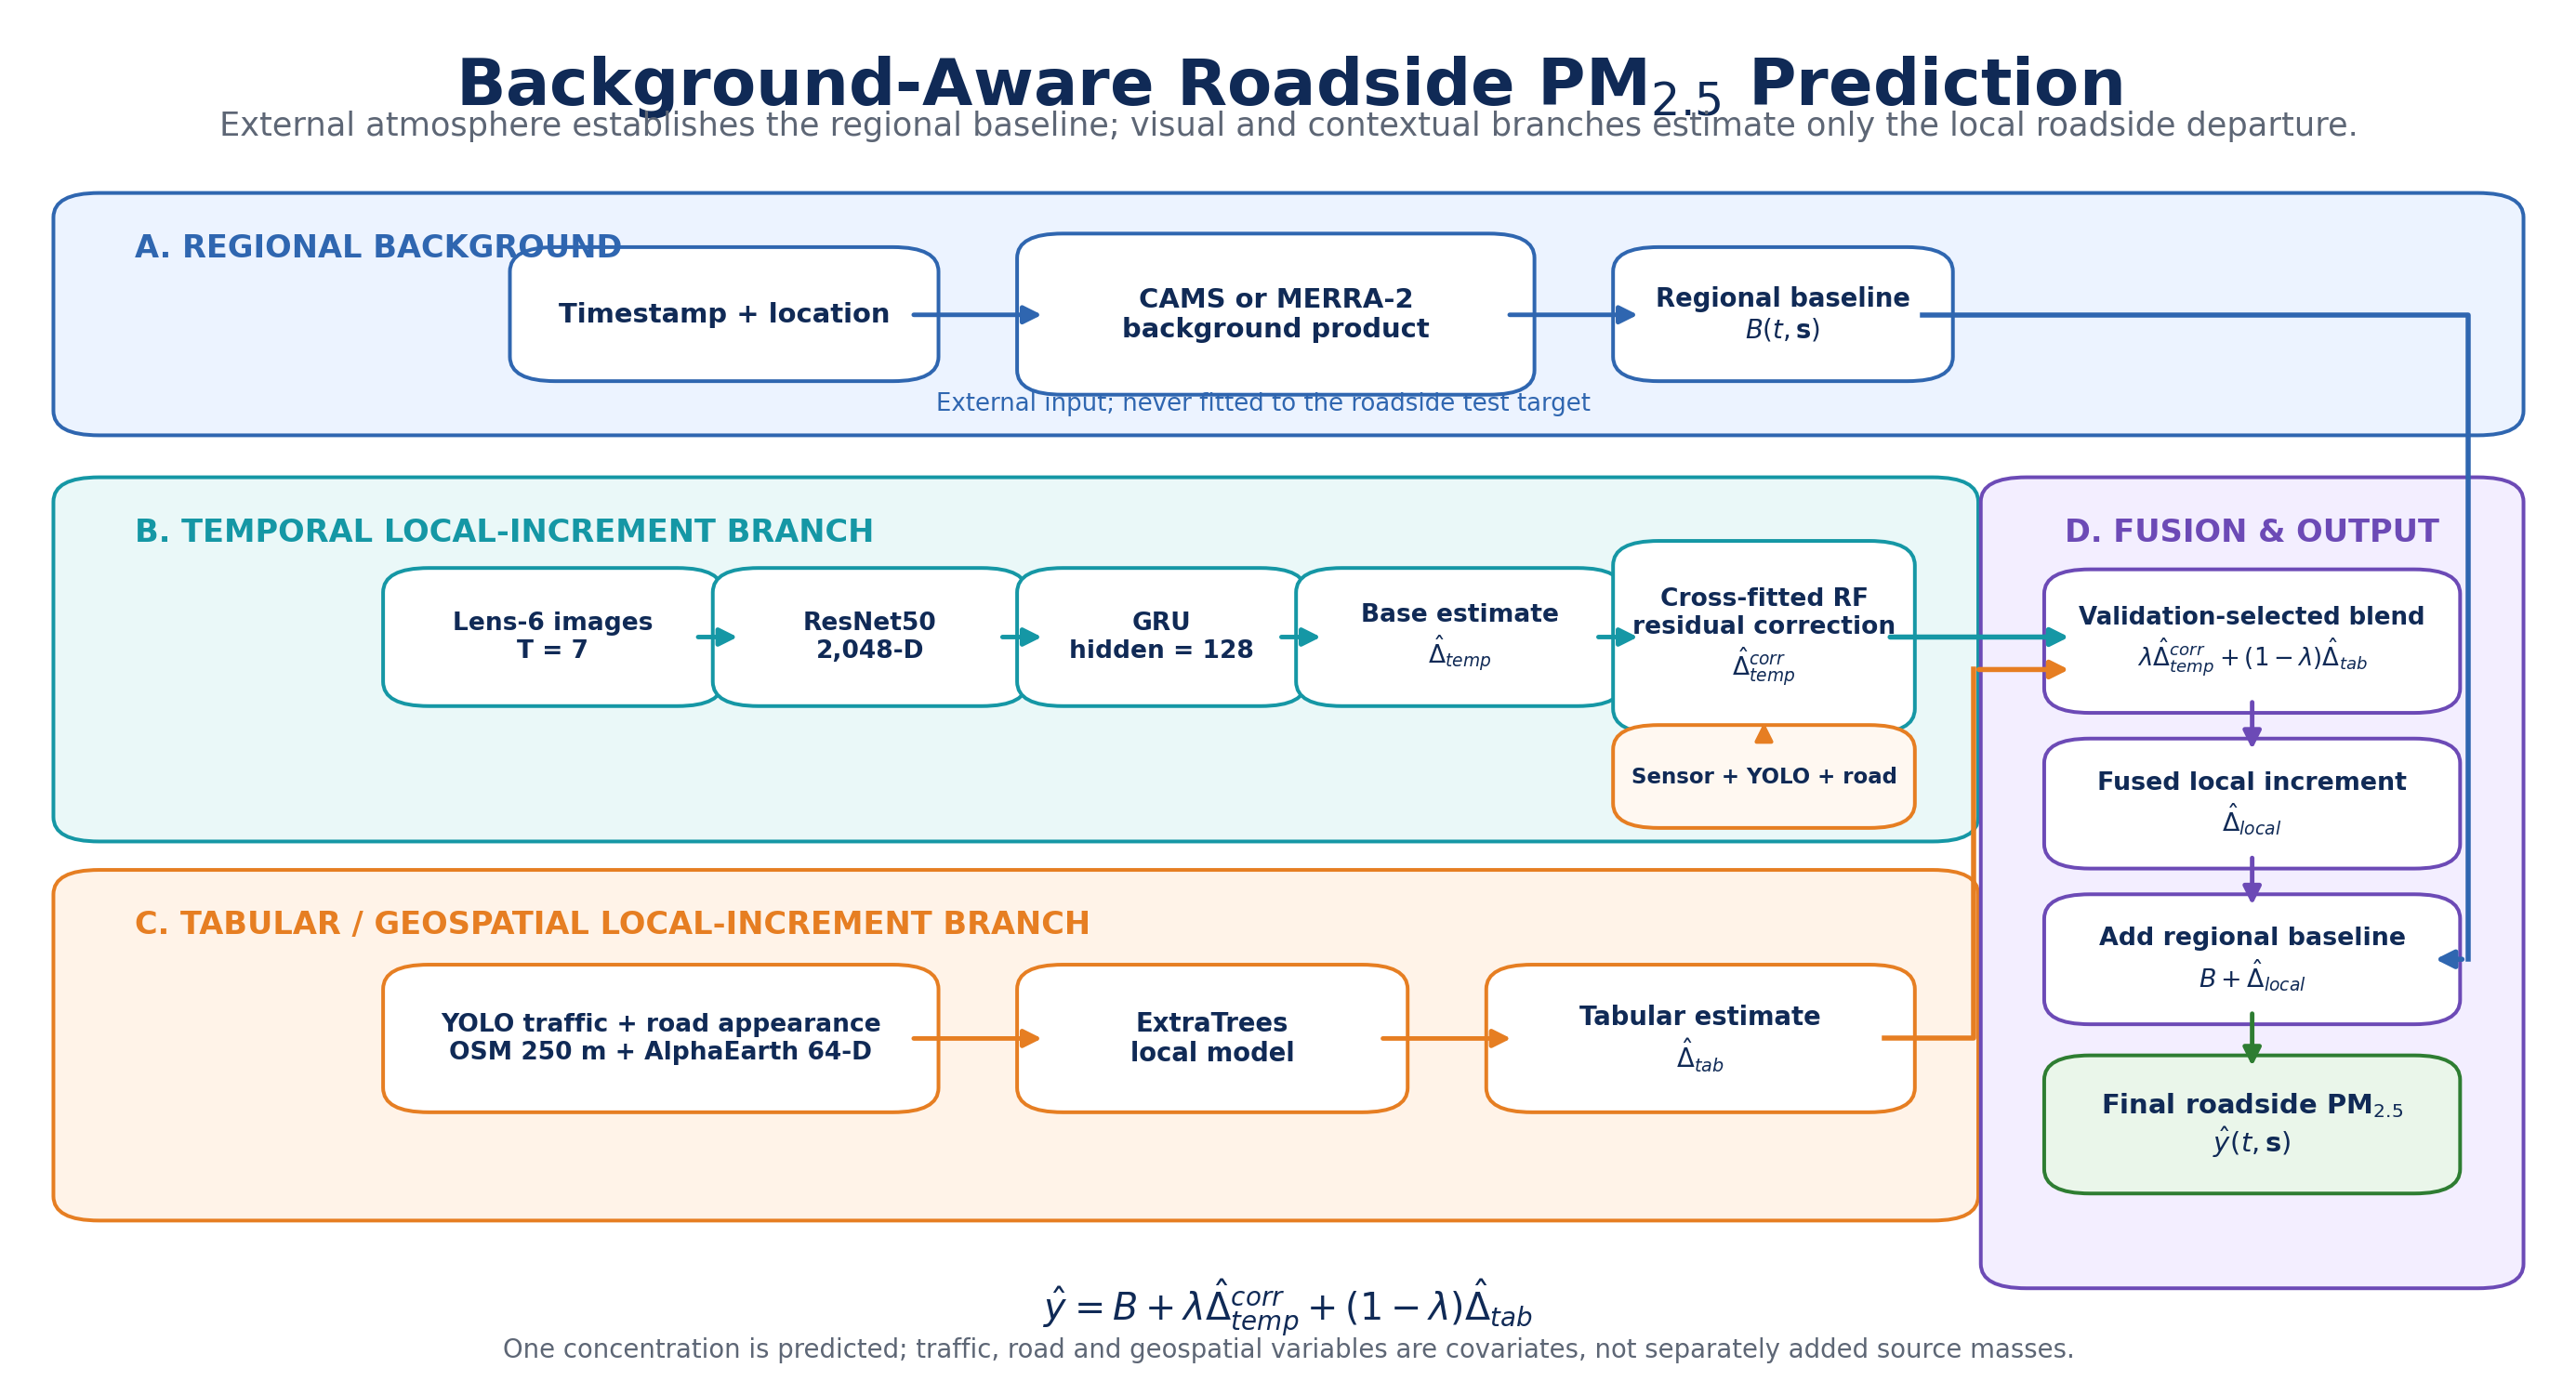
\includegraphics[width=\textwidth]{current_architecture.png}
  \caption{Current background-plus-local-increment architecture. Traffic, road,
  OSM and AlphaEarth are covariates for the local departure; their predictions
  are not separately added as physical source masses.}
  \label{fig:architecture}
\end{figure}

\section{Architecture 2: image-atmosphere early fusion}
The professor-proposed alternative combined a target-frame front/rear ResNet50
embedding with 22 atmospheric features. The image embedding was reduced by
train-only randomised PCA (requested 64 components), concatenated with CAMS,
MERRA-2 and ERA5 variables and passed to an ExtraTrees regressor. A 90\%
validation-absolute-residual conformal interval quantified uncertainty.

This tests predictive multimodal fusion, but it does not isolate ``pure
atmospheric PM'' because the target remains the roadside sensor. It also does
not estimate road and vehicle source contributions. The experiment was run on
both TRAQID and MUMMA under complete-date holdout.

\chapter{Experimental Design and Validation}

\section{Random row split}
Rows are shuffled between training and test. Adjacent ten-second observations
and the same dates occur in both partitions. This protocol answers: ``Can the
model interpolate among highly similar observations from the same collection
distribution?'' It does not answer: ``Will the model work on a new date?''

\section{Random sequence split after window construction}
T=7 or T=9 windows are first built with stride one and then shuffled. Adjacent
windows share most raw frames. For the five-day T=7 experiment:
\begin{itemize}
  \item 6,451 of 6,873 raw samples appeared in multiple partitions;
  \item 5,142 raw samples overlapped training and test;
  \item 1,287 of 1,309 test target frames appeared as training context; and
  \item the target/context leakage fraction was 98.32\%.
\end{itemize}

\begin{figure}[H]
  \centering
  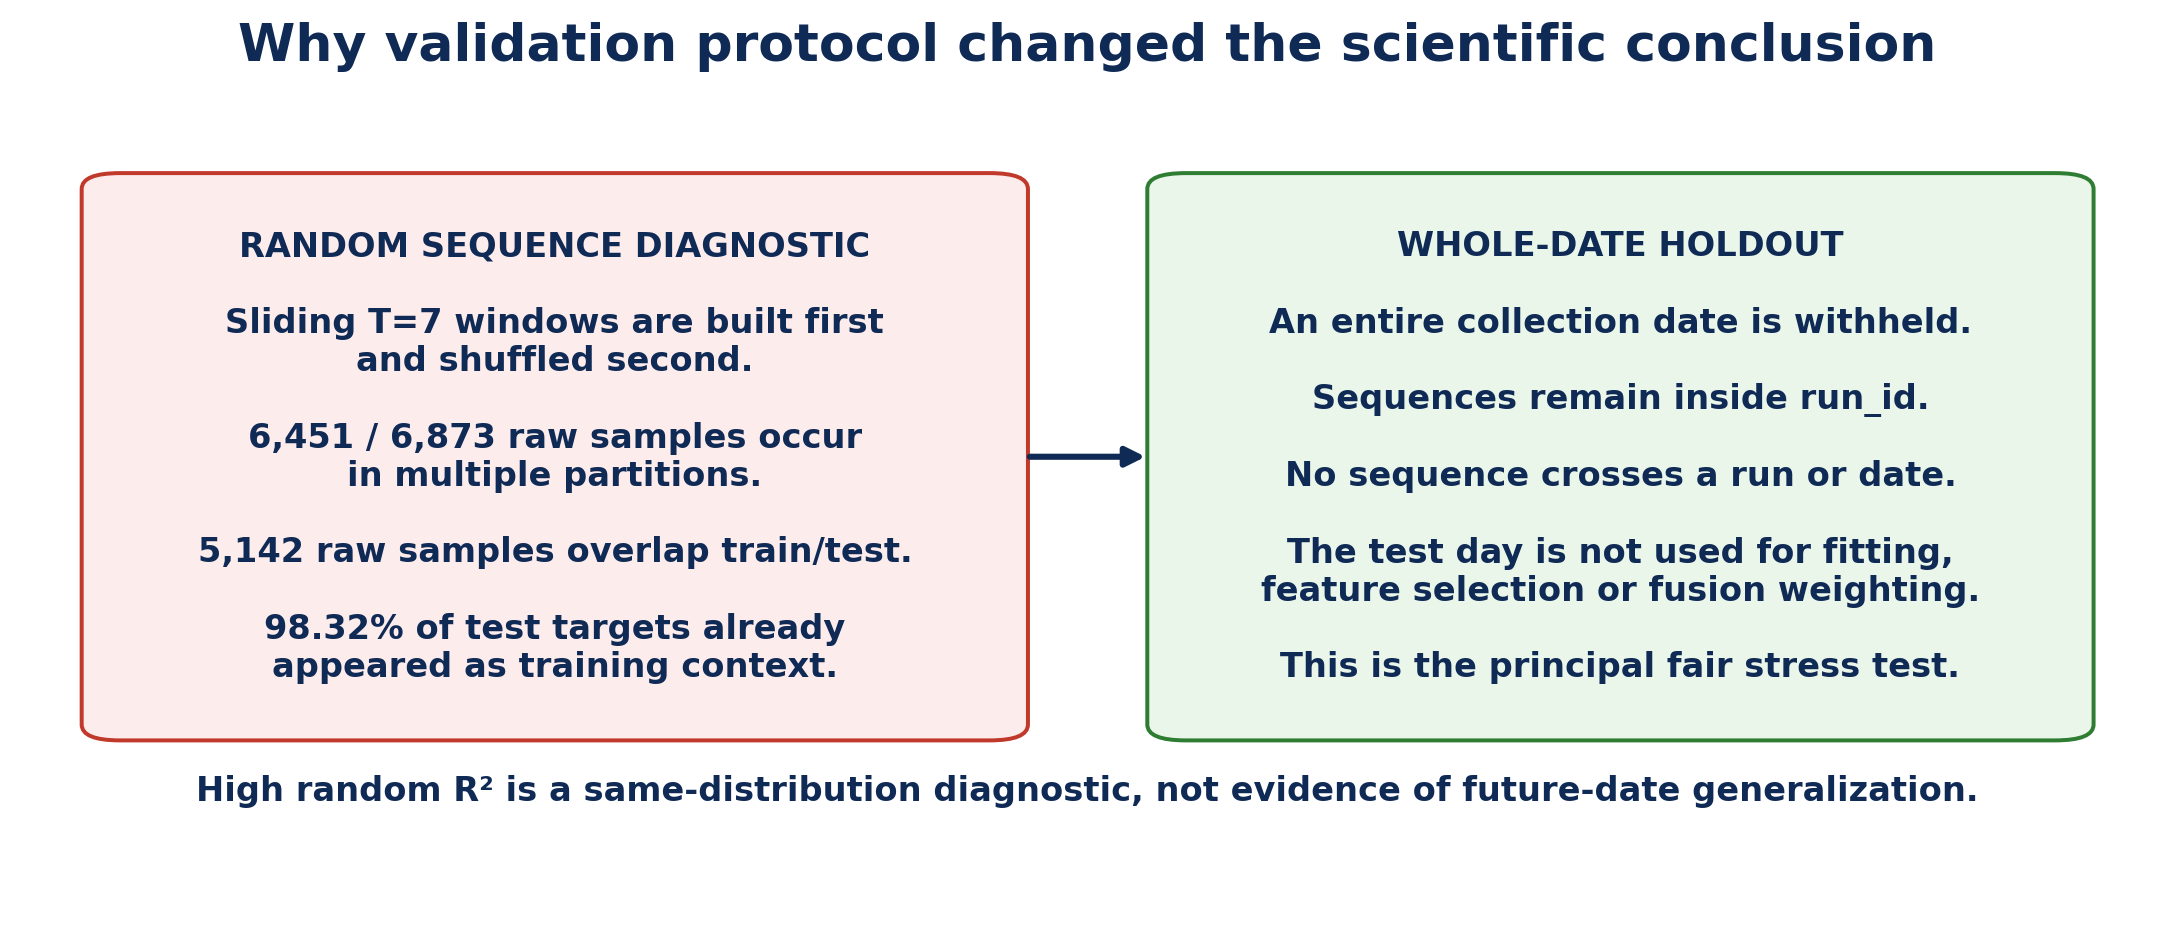
\includegraphics[width=0.96\textwidth]{validation_protocols.png}
  \caption{Contrast between the random overlapping-window diagnostic and the
  whole-date holdout used for fair evaluation.}
  \label{fig:validation}
\end{figure}

\section{Whole-date outer holdout}
Each of the five dates is held out in turn. Training uses the other dates;
sequences remain within \texttt{run\_id}. Each row receives one outer-test
prediction from a model that did not train on its date. Pooled metrics are
computed over the concatenated predictions, while fold metrics reveal
date-specific stability.

\section{Nested selection and cross-fitting}
For each outer fold, hyperparameters or fusion weights are chosen from an
outer-validation partition only. Residual correction on the validation date is
cross-fitted by run to avoid training and scoring the correction on the same
residuals. The outer-test date is untouched until the architecture and weight
are frozen.

Even this protocol remains \emph{exploratory} at the project level because the
same five dates informed multiple architecture decisions during two months of
development. Confirmatory evidence requires new dates collected after the
pipeline is frozen.

\section{Pooled versus per-date \Rtwo}
Pooled \Rtwo\ uses one global mean:
\begin{equation}
  R^2_{\mathrm{pooled}}
  =1-\frac{\sum_d\sum_i(y_{di}-\hat y_{di})^2}
           {\sum_d\sum_i(y_{di}-\bar y)^2}.
\end{equation}
Its denominator includes between-date baseline variation. Mean fold \Rtwo\
instead computes \Rtwo\ within each day and averages the five values. A model
can therefore have positive pooled \Rtwo\ by predicting high days versus low
days while still performing poorly relative to each day's local mean. Both
statistics are reported.

\cautionbox{No random-window result in this report is labelled as future-date
generalisation. Whole-date results are fair stress tests, but final deployment
claims still require untouched future collection dates.}

\chapter{PM$_{2.5}$ Prediction Results}

\section{Historical TRAQID random-window progression}
Table~\ref{tab:traqidrandom} reconstructs the result shown in the historical
presentation. Each improvement was measured on the same overlap-contaminated
random-window benchmark.

\begin{table}[H]
  \centering
  \caption{Historical TRAQID random-window result progression.}
  \label{tab:traqidrandom}
  \begin{tabular}{lrrr}
    \toprule
    Variant & MAE (\ugm) & RMSE (\ugm) & \Rtwo\\
    \midrule
    Single ResNet50-GRU & 5.991 & 10.359 & 0.951\\
    Tuned residual using base prediction & 5.440 & 9.847 & 0.956\\
    Three-model base ensemble & 5.113 & 9.434 & 0.960\\
    OOF ExtraTrees residual, unclipped & 4.234 & 8.867 & 0.964\\
    OOF ExtraTrees residual, clipped $\pm12.5$ & \textbf{4.212} &
      \textbf{8.717} & \textbf{0.966}\\
    \bottomrule
  \end{tabular}
\end{table}

Later TRAQID date-held-out ResNet50-GRU folds obtained \Rtwo\ 0.249, -0.079,
-0.883, -0.313 and -0.307. The gap between these values and 0.966 is evidence
of date shift and overlap effects, not a contradiction in the implementation.

\section{TRAQID matched direct and background random tests}
A later matched random experiment compared direct \pmtwo, CAMS plus local
increment, MERRA-2 plus local increment and GEOS-CF. The same 3,983 test
sequences and 714 correction features were used.

\begin{table}[H]
  \centering
  \caption{Selected TRAQID matched random-sequence results. These remain random
  diagnostics.}
  \label{tab:traqidmatchedrandom}
  \begin{tabular}{llrrr}
    \toprule
    Framework & Correction & MAE & RMSE & \Rtwo\\
    \midrule
    Direct \pmtwo & Random Forest & 6.583 & 11.171 & 0.9413\\
    CAMS + local increment & ExtraTrees & 6.197 & 10.882 & 0.9443\\
    MERRA-2 + local increment & Random Forest & 5.948 & 10.657 & 0.9466\\
    GEOS-CF + local increment & ExtraTrees & 6.779 & 11.264 & 0.9403\\
    \bottomrule
  \end{tabular}
\end{table}

MERRA-2 was best in the matched random comparison, although the uncorrected
MERRA-2 image-base row had the lowest MAE (5.878) while its \Rtwo\ was slightly
lower (0.9460). Metric rankings can differ because MAE and RMSE weight errors
differently.

\section{TRAQID whole-date background ensembles}
The same background concept did not transfer as strongly to TRAQID whole-date
holdout. The MERRA-2 fixed 50:50 temporal-tabular diagnostic was best with MAE
29.32, RMSE 43.18 and pooled \Rtwo\ 0.147. Its mean fold \Rtwo\ was only 0.047.
The validation-selected MERRA-2 ensemble reached pooled \Rtwo\ 0.036. CAMS
fixed 50:50 reached 0.076. These results demonstrate that an architecture can
help one dataset and fail to provide the same benefit under a different route,
sensor, background or date distribution.

\section{Two-day MUMMA prototyping}
In random overlapping sequences, the image-base \Rtwo\ increased from 0.679 at
T=3 to 0.797 at T=7 and 0.828 at T=9. Leakage increased at the same time. At
T=9, 99.27\% of test target frames had already appeared as training context. A
causal trailing-three-row smoothed target produced MAE 3.875, RMSE 6.033 and
\Rtwo\ 0.958. This was a useful upper-bound experiment but not a deployment
score because the target was smoother and the split was heavily contaminated.

The two-day whole-date test was much worse. The best T=7 visual correction had
RMSE 41.00 and \Rtwo\ -0.542. With only two dates, there was no independent
nested date for correction-model selection.

\section{Five-day image backbone and view comparison}
Table~\ref{tab:backbones} reports mean performance over five held-out dates.
Changing the CNN or recurrent cell did not solve date shift.

\begin{table}[H]
  \centering
  \caption{Five-day fair image-model comparison. \Rtwo\ is the mean of the five
  date-specific values.}
  \label{tab:backbones}
  \begin{adjustbox}{max width=\textwidth}
  \begin{tabular}{lrrrr}
    \toprule
    Image model & Mean MAE & Mean RMSE & Mean \Rtwo & Worst RMSE\\
    \midrule
    ResNet50-GRU T7, lens 6 & 38.72 & 47.29 & -1.385 & 80.70\\
    ResNet50-GRU T7, mean 1/2/6 & 38.58 & 47.43 & -1.319 & 78.30\\
    ResNet50-GRU T7, concat 1/2/6 & 39.05 & 47.54 & -1.323 & 82.65\\
    ConvNeXt-tiny-GRU T7, concat & 39.63 & 47.74 & -1.329 & 82.16\\
    ResNet50-LSTM T7, concat & 39.95 & 48.46 & -1.394 & 85.26\\
    Robust ResNet50-GRU T7, concat & 40.43 & 48.53 & -1.471 & 87.19\\
    MobileNetV2-GRU T7, concat & 43.04 & 50.89 & -1.742 & 92.77\\
    \bottomrule
  \end{tabular}
  \end{adjustbox}
\end{table}

Lens 6 was retained for the structured temporal branch because it was a
competitive single view, reduced dimensionality and showed the most consistent
road-facing content. The attempted five-day random ResNet50-LSTM run contained
sequence and audit files but no final trained metrics, so it was marked
incomplete rather than inferred.

\section{Five-day random-sequence diagnostics}
\begin{table}[H]
  \centering
  \caption{Selected five-day random-sequence results. All have temporal overlap
  and are not future-date scores.}
  \label{tab:fivedayrandom}
  \begin{adjustbox}{max width=\textwidth}
  \begin{tabular}{lrrr}
    \toprule
    Base and correction & MAE & RMSE & \Rtwo\\
    \midrule
    Lens-6 ResNet50-GRU T7 + sensor/visual RF & 10.105 & 19.608 & 0.852\\
    Concat ResNet50-GRU T7 + sensor/visual RF & 9.328 & 19.308 & 0.856\\
    Concat ResNet50-GRU T9 + sensor/visual RF & 8.292 & 25.251 & 0.776\\
    ConvNeXt-tiny-GRU T7 + sensor/visual RF & 8.951 & 18.537 & 0.867\\
    ConvNeXt-tiny-GRU T7 + sensor/AlphaEarth ET & 8.825 & 18.592 & 0.867\\
    CAMS + ResNet50-GRU T7 + sensor/visual/AE ET & 9.856 & 20.032 & 0.845\\
    CAMS + same + OSM ET & 9.787 & 19.897 & 0.847\\
    \bottomrule
  \end{tabular}
  \end{adjustbox}
\end{table}

OSM improved the matched CAMS random result by only 0.134 RMSE and 0.002 \Rtwo.
Five extreme test samples in the final OSM random run had RMSE 188.90 compared
with 17.58 for inliers, showing that a small number of peaks dominated the
overall squared error.

\begin{figure}[H]
  \centering
  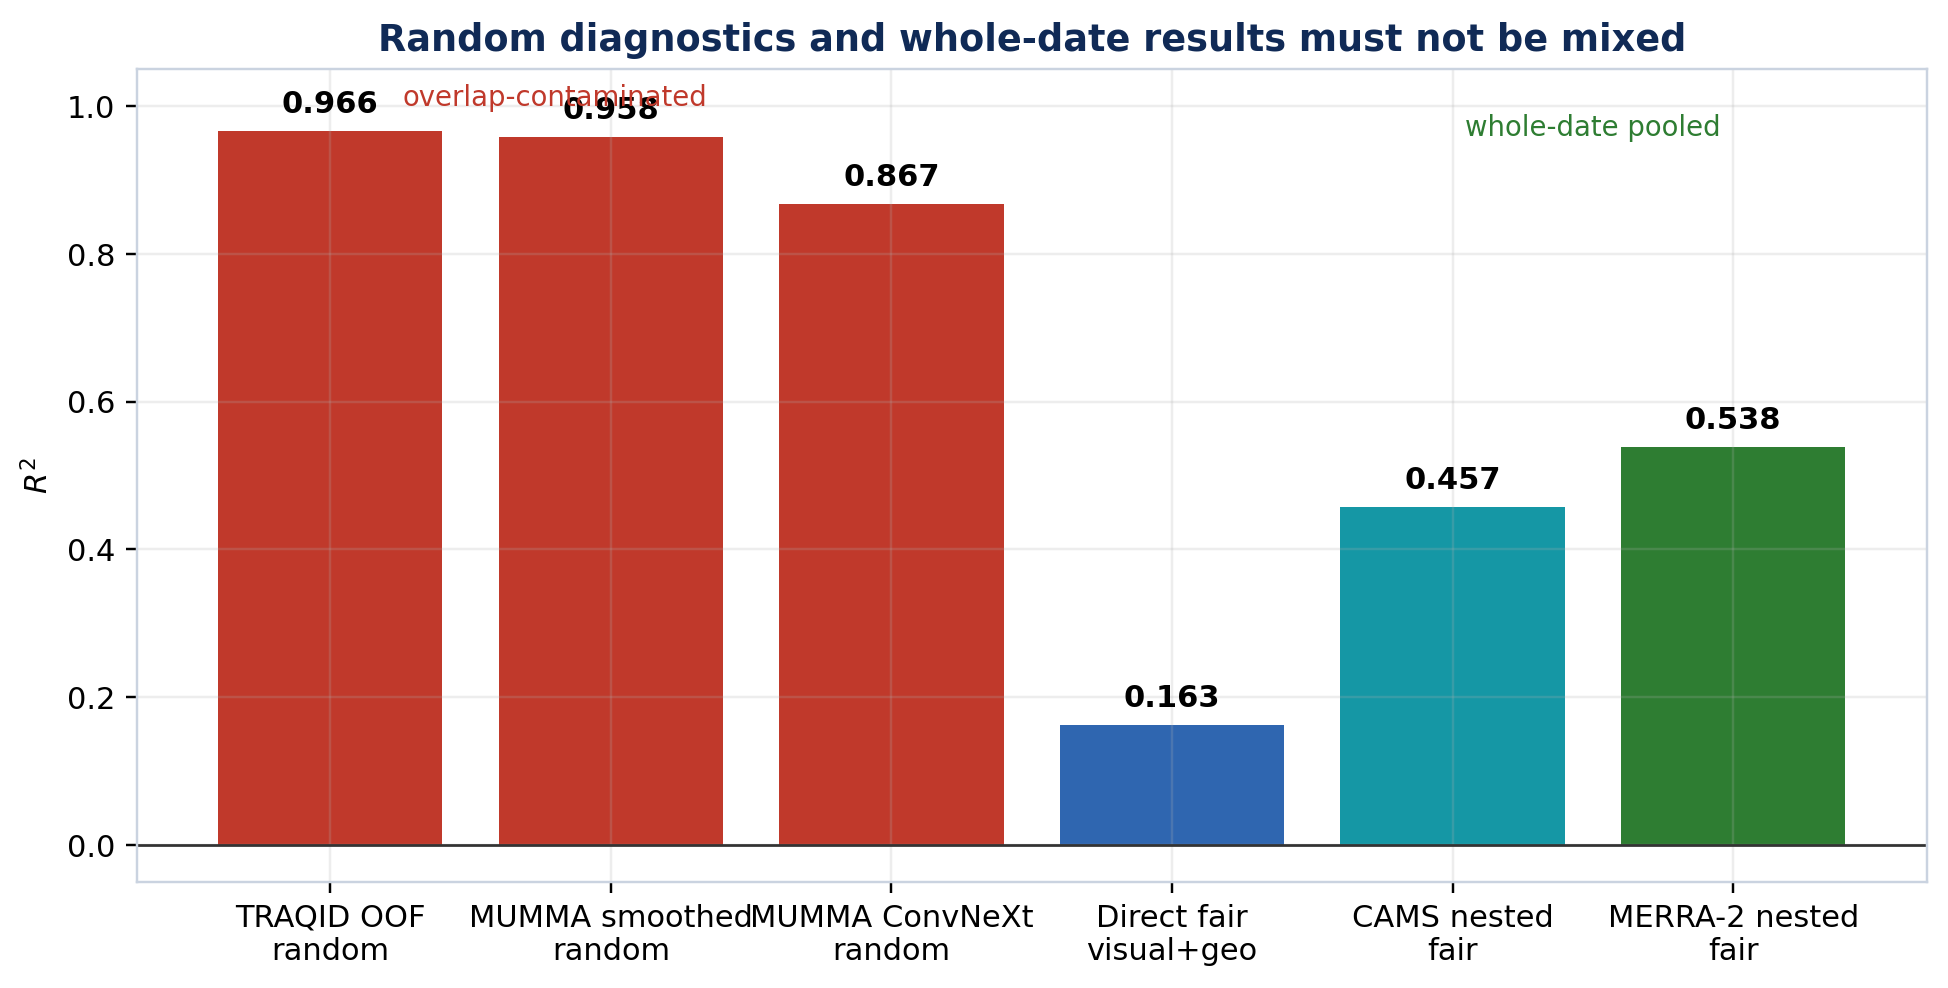
\includegraphics[width=0.86\textwidth]{random_vs_fair_r2.png}
  \caption{Representative random and whole-date pooled results. The bars are
  displayed together only to show the validation gap; they are not directly
  comparable claims.}
  \label{fig:randomfair}
\end{figure}

\section{Five-day direct tabular models}
The direct tabular benchmark compared Ridge, Random Forest, ExtraTrees and
HistGradientBoosting across feature groups.
\begin{itemize}
  \item The best random-row diagnostic used 24 sensor/met/gas/time/mobility
        features with ExtraTrees: MAE 8.43, RMSE 29.83, \Rtwo\ 0.730 and
        Spearman 0.960.
  \item The best complete fair visual/geospatial row used 192
        YOLO/road/OSM/AlphaEarth features with HistGradientBoosting: MAE 34.96,
        RMSE 47.74, pooled \Rtwo\ 0.163 and Spearman 0.509.
  \item Without OSM, visual/road/AlphaEarth Ridge reached RMSE 48.40 and pooled
        \Rtwo\ 0.140.
  \item Nested top-30 feature selection was worse than keeping all 192
        features: RMSE 48.87 versus 47.59 and \Rtwo\ 0.123 versus 0.168.
\end{itemize}
This result suggests distributed information across correlated feature groups;
a hard importance cutoff discarded useful complementary variables.

\section{Direct image plus residual correction}
The best fair direct image-plus-residual configuration was ResNet50-GRU T7 with
sensor/AlphaEarth Random Forest correction: MAE 32.82, RMSE 47.33 and pooled
\Rtwo\ 0.187. Sensor/visual correction reached \Rtwo\ 0.175. ConvNeXt correction
reached 0.136, while the robust ResNet variant reached only 0.032. Correction
candidates had been compared after observing outer-test results, so this stage
was exploratory rather than confirmatory.

\section{CAMS background plus local increment}
The CAMS decomposition was the first major improvement under whole-date
evaluation:
\begin{table}[H]
  \centering
  \caption{CAMS whole-date local-increment results.}
  \label{tab:cams}
  \begin{tabular}{lrrr}
    \toprule
    Model & MAE & RMSE & Pooled \Rtwo\\
    \midrule
    Tabular visual/road/AlphaEarth ExtraTrees & 27.59 & 39.59 & 0.425\\
    Tabular + OSM ExtraTrees & 27.52 & 39.56 & 0.425\\
    Temporal ResNet50-GRU + sensor/visual RF & 26.26 & 39.89 & 0.423\\
    Nested ensemble, validation-selected, no OSM & 25.281 & 38.666 & 0.457\\
    Nested ensemble, fixed 50:50 diagnostic & 25.275 & 38.288 & 0.468\\
    Nested ensemble, validation-selected, OSM & 25.456 & 38.780 & 0.454\\
    \bottomrule
  \end{tabular}
\end{table}
OSM was useful and interpretable in the standalone tabular branch but slightly
worsened the full selected ensemble. The no-OSM validation-selected CAMS model
was therefore the earlier frozen candidate.

\section{MERRA-2 refinement}
MERRA-2 provided the strongest background signal tested on five-day MUMMA.
The standalone MERRA-2 plus YOLO/road/OSM/AlphaEarth ExtraTrees model achieved
MAE 23.49, RMSE 35.01 and pooled \Rtwo\ 0.550 over all 6,873 rows.

The nested ensemble used 6,543 sequence-aligned test rows:
\begin{table}[H]
  \centering
  \caption{MERRA-2 nested whole-date ensemble results.}
  \label{tab:merra}
  \begin{tabular}{lrrrr}
    \toprule
    Method & $n$ & MAE & RMSE & Pooled \Rtwo\\
    \midrule
    Fixed equal weight diagnostic & 6,543 & \textbf{21.985} &
      \textbf{34.589} & \textbf{0.566}\\
    Tabular branch & 6,543 & 23.520 & 35.276 & 0.548\\
    Validation-selected weight & 6,543 & 22.580 & 35.689 & 0.538\\
    Temporal branch & 6,543 & 23.650 & 37.030 & 0.502\\
    \bottomrule
  \end{tabular}
\end{table}

\resultbox{The primary selection-valid MERRA-2 result is MAE 22.58 \ugm, RMSE
35.69 \ugm\ and pooled \Rtwo\ 0.538. The fixed 50:50 result is numerically
better but is labelled a diagnostic because that weight was not chosen by the
predefined validation rule.}

\begin{figure}[H]
  \centering
  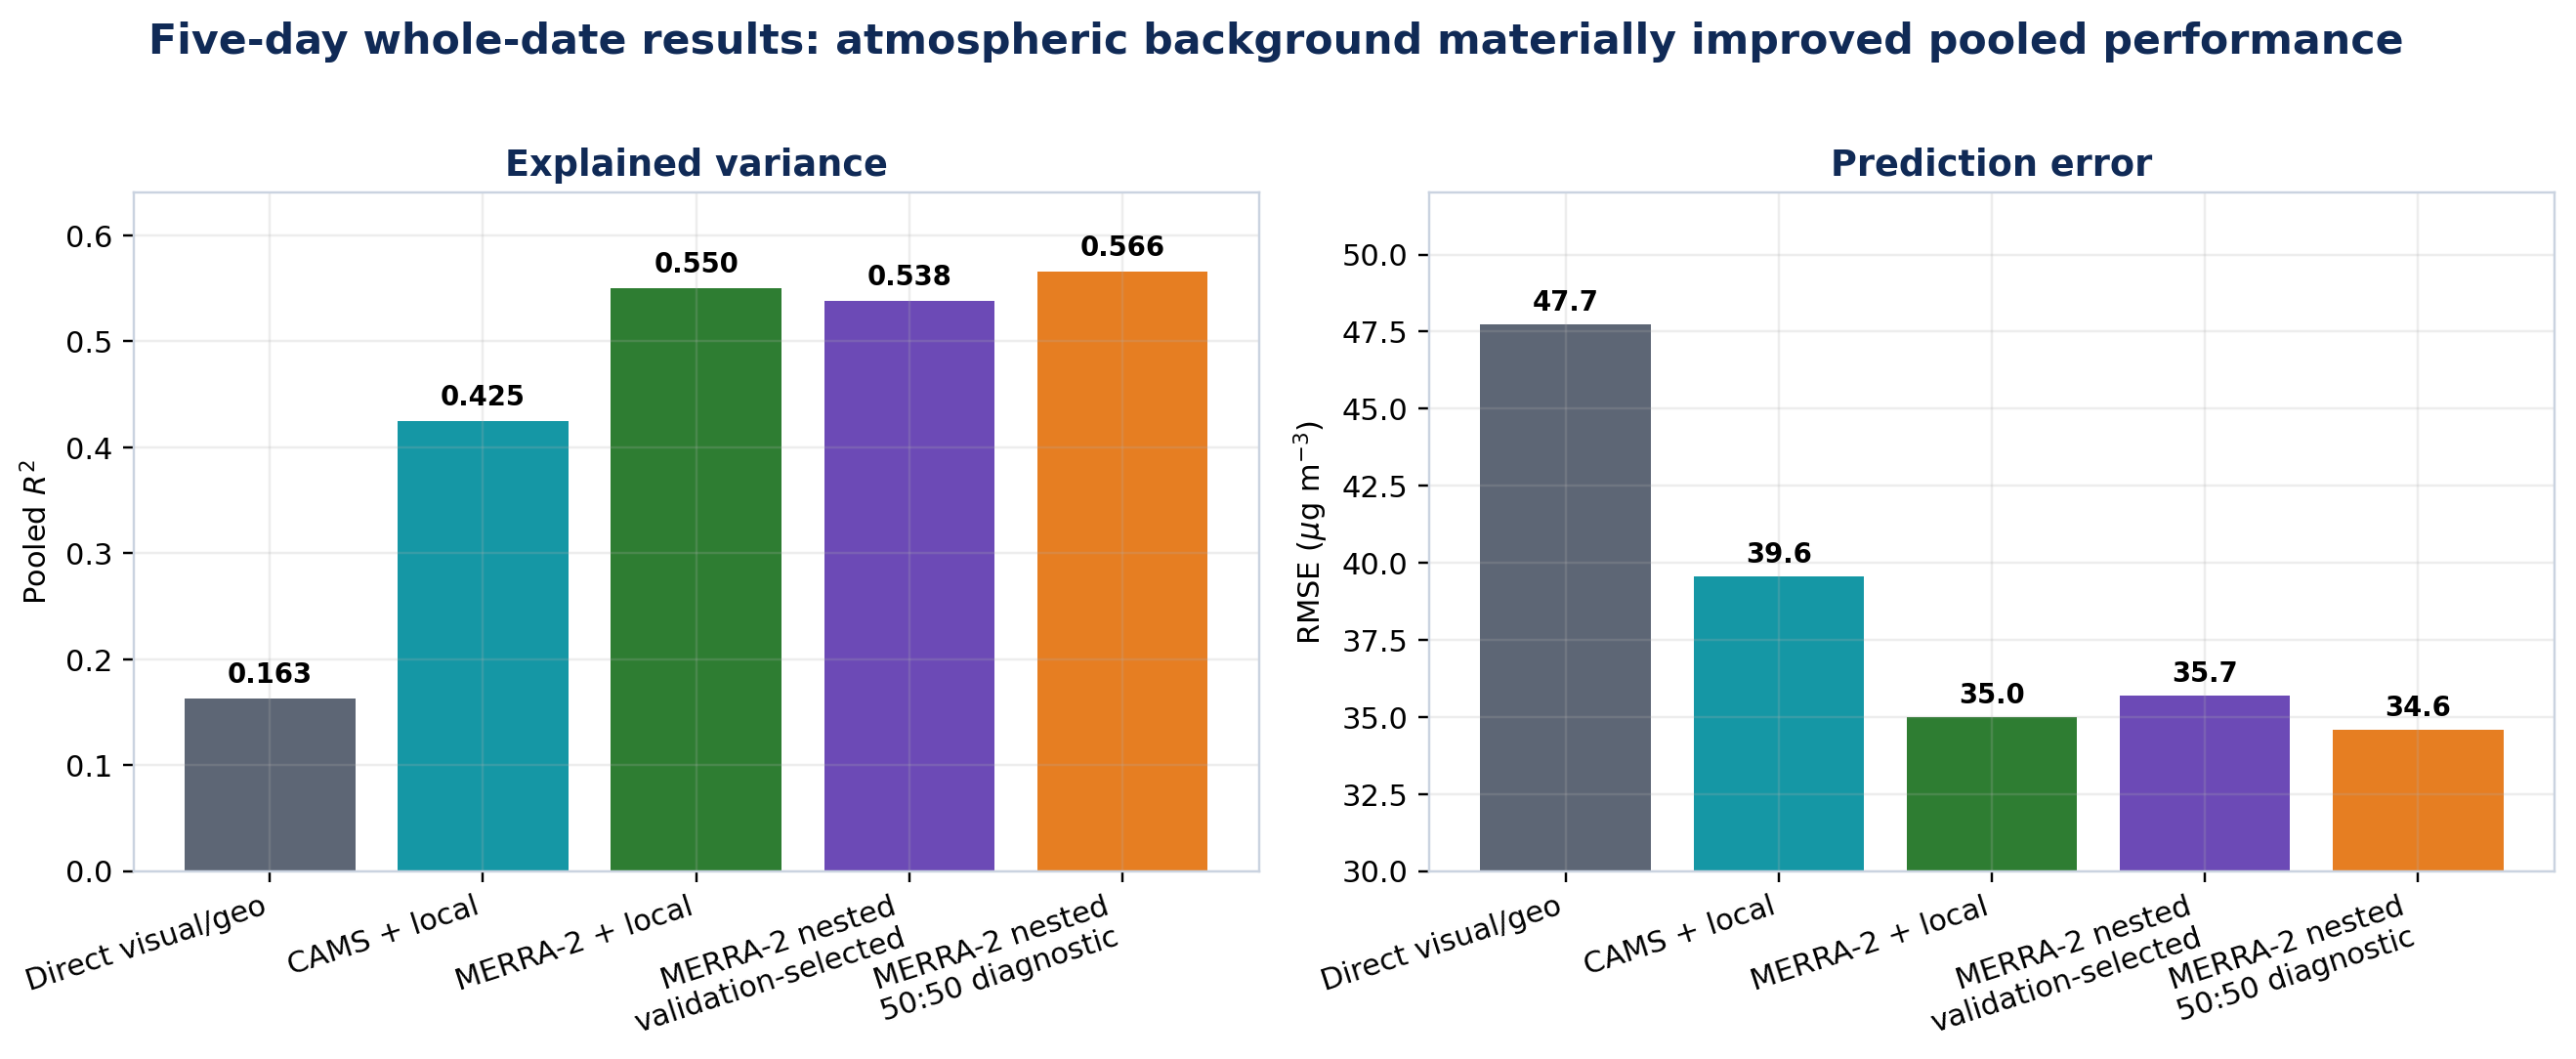
\includegraphics[width=0.98\textwidth]{background_model_comparison.png}
  \caption{Progression from direct whole-date modelling to CAMS and MERRA-2
  background-plus-local-increment models.}
  \label{fig:backgroundcompare}
\end{figure}

The selected temporal weights averaged 0.826 and ranged from 0.733 to 0.955.
However, the selected model's date-specific \Rtwo\ values were -0.791, -0.467,
-0.283, 0.277 and 0.232. Its mean fold \Rtwo\ was -0.207.

\begin{figure}[H]
  \centering
  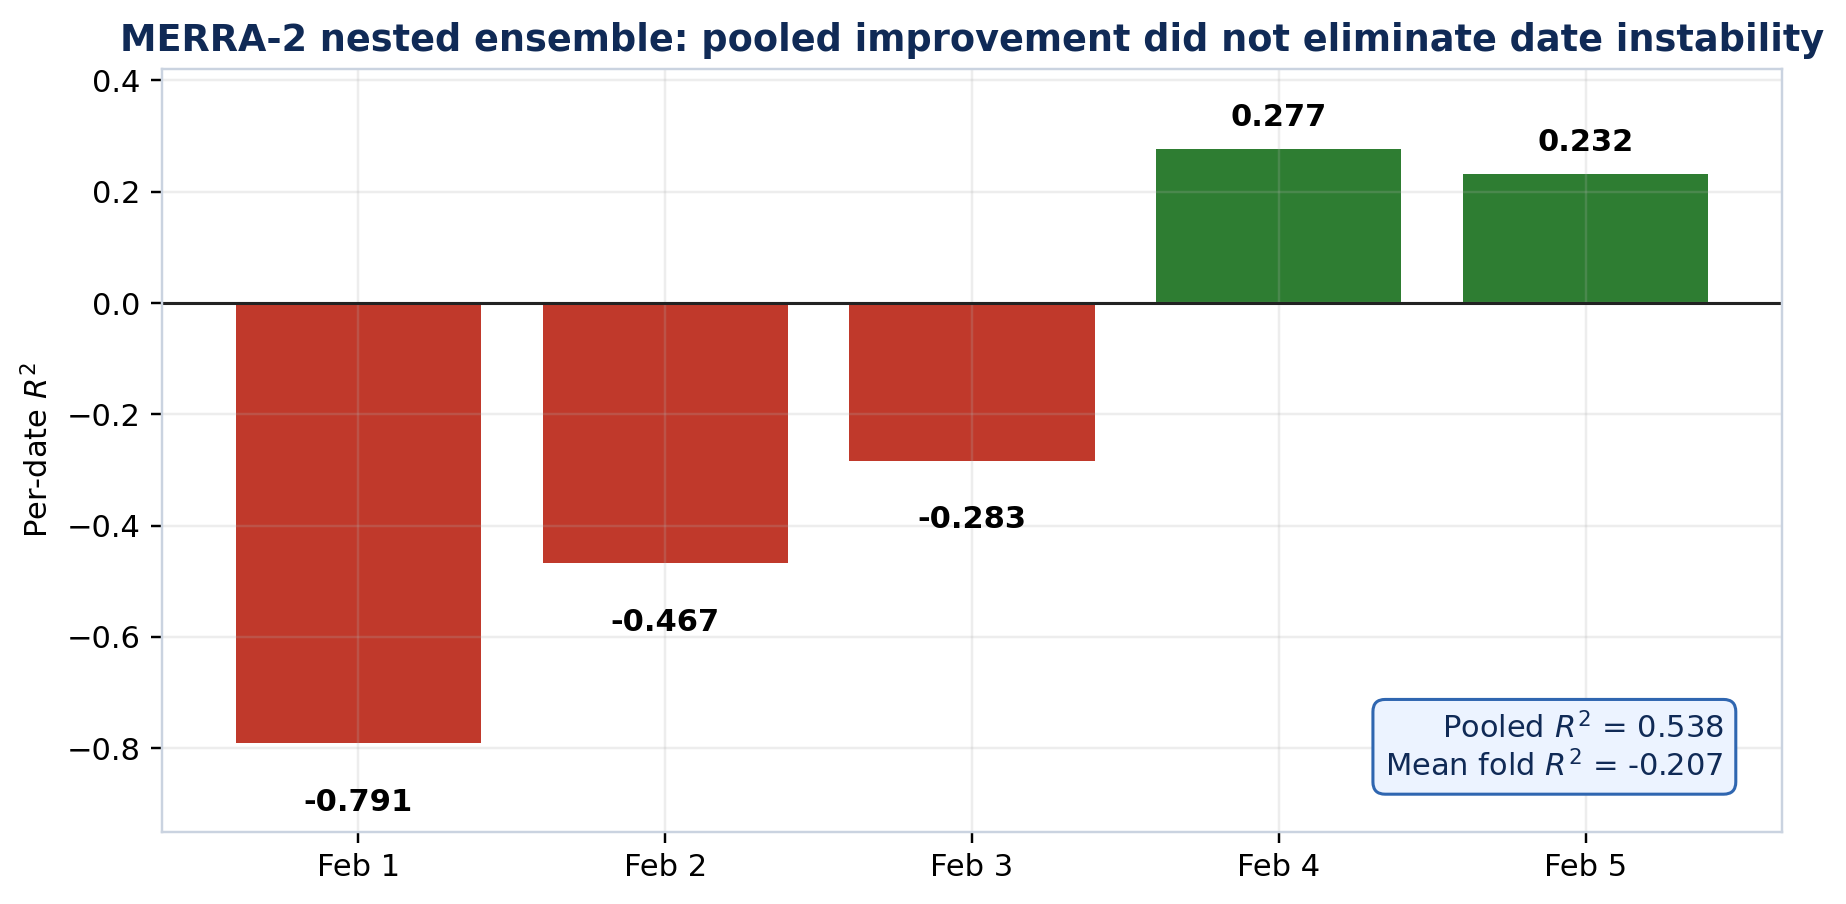
\includegraphics[width=0.84\textwidth]{merra_per_date_r2.png}
  \caption{Date-specific \Rtwo\ for the validation-selected MERRA-2 nested
  ensemble. Positive pooled performance coexists with unstable within-date
  prediction.}
  \label{fig:perdate}
\end{figure}

\section{Atmospheric source ablation}
A matched comparison showed:
\begin{table}[H]
  \centering
  \caption{Five-day pooled comparison of atmospheric backgrounds with the same
  local modelling concept.}
  \begin{tabular}{lrrr}
    \toprule
    Background framework & MAE & RMSE & Pooled \Rtwo\\
    \midrule
    Raw MERRA-2 + local & 23.484 & 35.031 & 0.550\\
    Mean CAMS/MERRA-2 + local & 24.872 & 36.558 & 0.509\\
    Raw CAMS + local & 27.606 & 39.586 & 0.425\\
    Nested calibrated atmosphere + local & 29.790 & 41.844 & 0.357\\
    Nested calibrated atmosphere only & 34.305 & 46.413 & 0.209\\
    \bottomrule
  \end{tabular}
\end{table}
Target-fitted atmospheric calibration did not help and was scientifically less
attractive because it introduced dependence on the roadside target. The raw,
externally available MERRA-2 background was therefore preferred.

\section{Architecture 2 results}
Architecture 2 combined image and atmospheric features early in one ExtraTrees
model. On MUMMA, atmosphere-only and early fusion were almost identical:

\begin{table}[H]
  \centering
  \caption{Architecture-2 whole-date results.}
  \label{tab:architecture2}
  \begin{tabular}{llrrr}
    \toprule
    Dataset & Variant & MAE & RMSE & Pooled \Rtwo\\
    \midrule
    \multirow{3}{*}{MUMMA}
      & Atmosphere only & 32.288 & 45.822 & 0.229\\
      & Early fusion & 32.498 & 45.805 & 0.230\\
      & Image only & 43.289 & 55.745 & -0.141\\
    \midrule
    \multirow{3}{*}{TRAQID}
      & Atmosphere only & 31.200 & 45.935 & 0.035\\
      & Early fusion & 32.192 & 46.832 & -0.003\\
      & Image only & 33.025 & 49.382 & -0.115\\
    \bottomrule
  \end{tabular}
\end{table}

\begin{figure}[H]
  \centering
  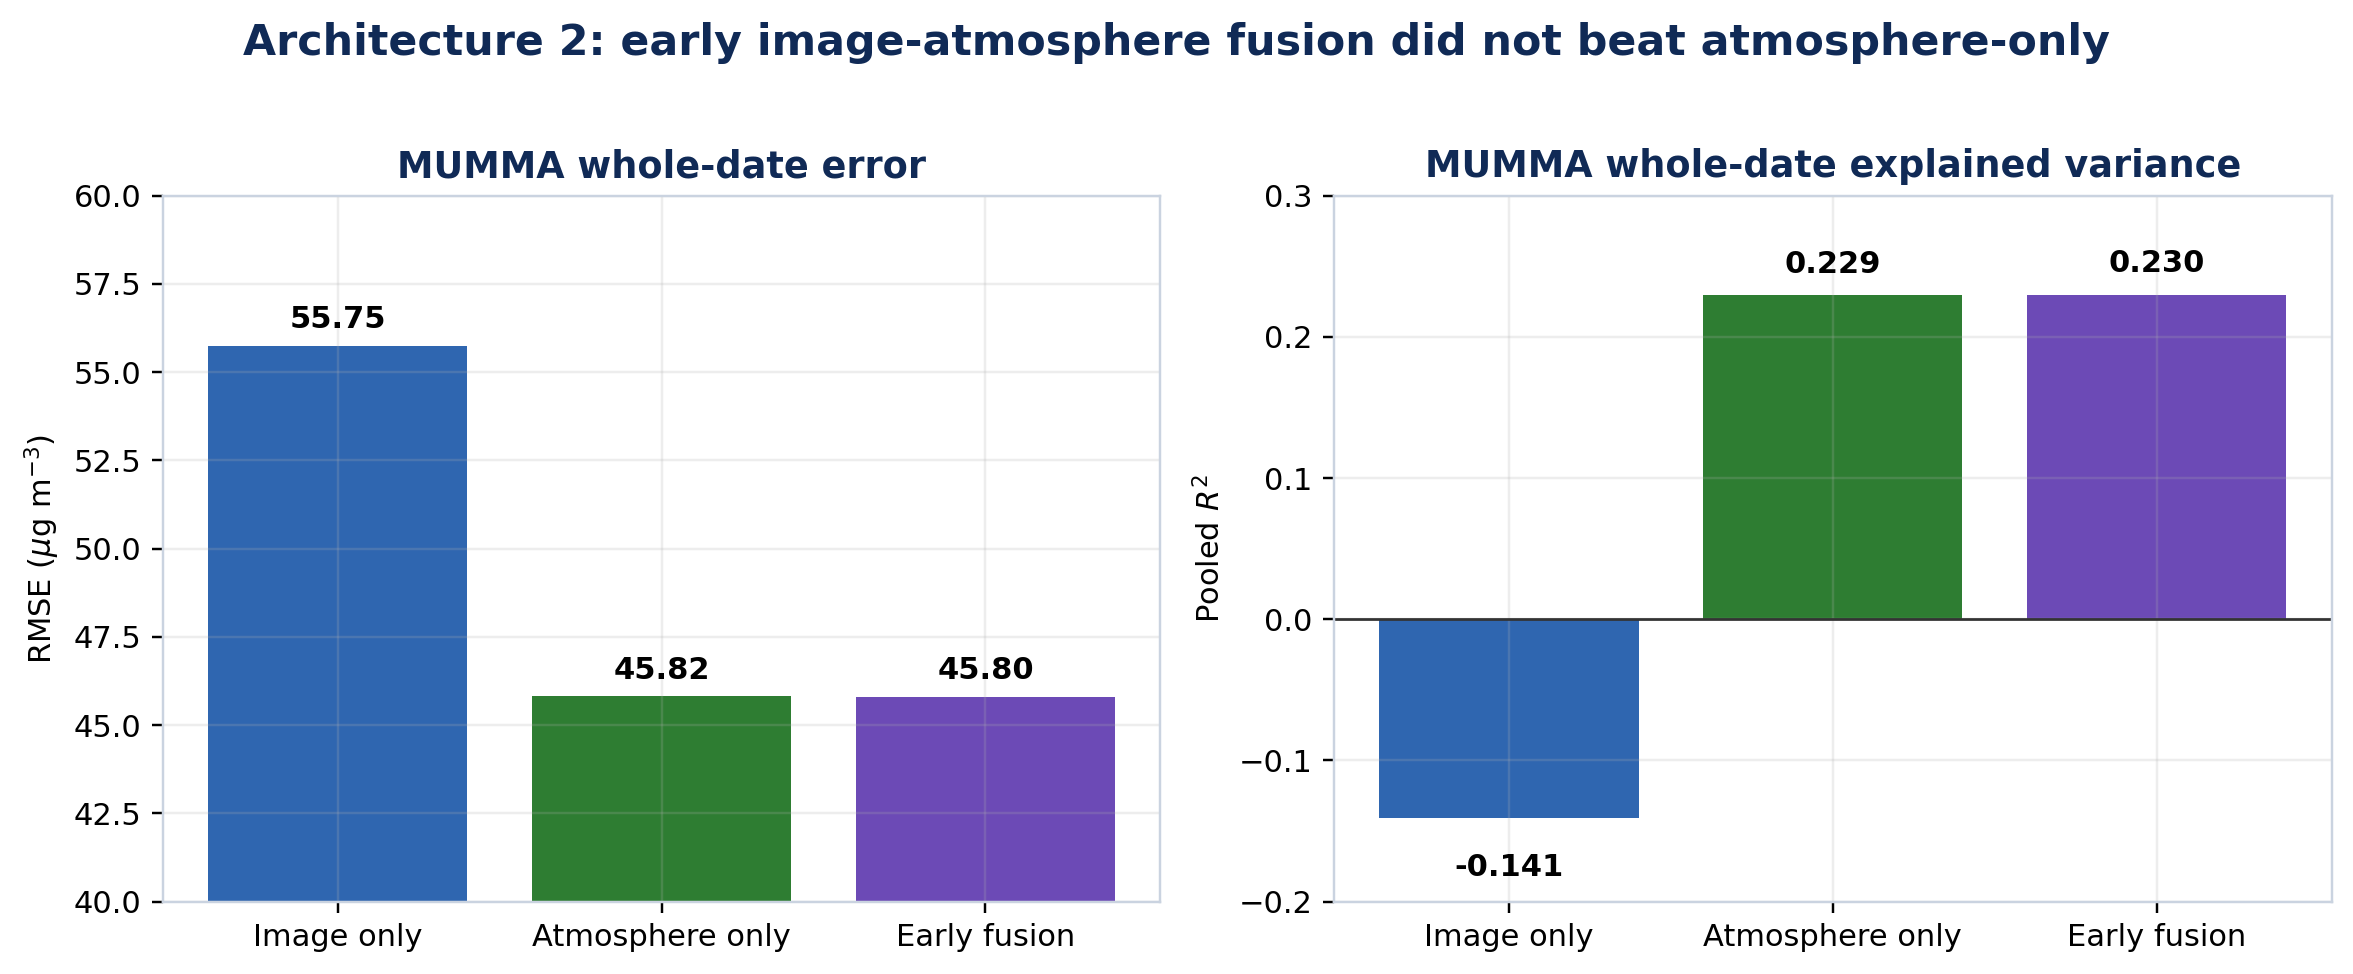
\includegraphics[width=0.88\textwidth]{architecture2_results.png}
  \caption{MUMMA architecture-2 ablation. The image embedding added almost no
  value over atmospheric fields in early fusion.}
  \label{fig:architecture2result}
\end{figure}

This result does not invalidate images. It shows that a single target-frame PCA
embedding concatenated with coarse atmosphere was not the right inductive bias
for these five dates. The structured background/local model performed better
because it assigned different roles to regional background and local evidence.

\section{Uncertainty quantification}
Validation absolute-residual conformal intervals were added without using
outer-test targets for calibration. For the MERRA-2 experiment, the nominal
coverage was 90\%. Empirical coverage ranged from 0.761 for the temporal branch
to 0.850 for the tabular branch; the validation-selected ensemble covered 0.776
with mean interval width 63.14 \ugm.

\begin{figure}[H]
  \centering
  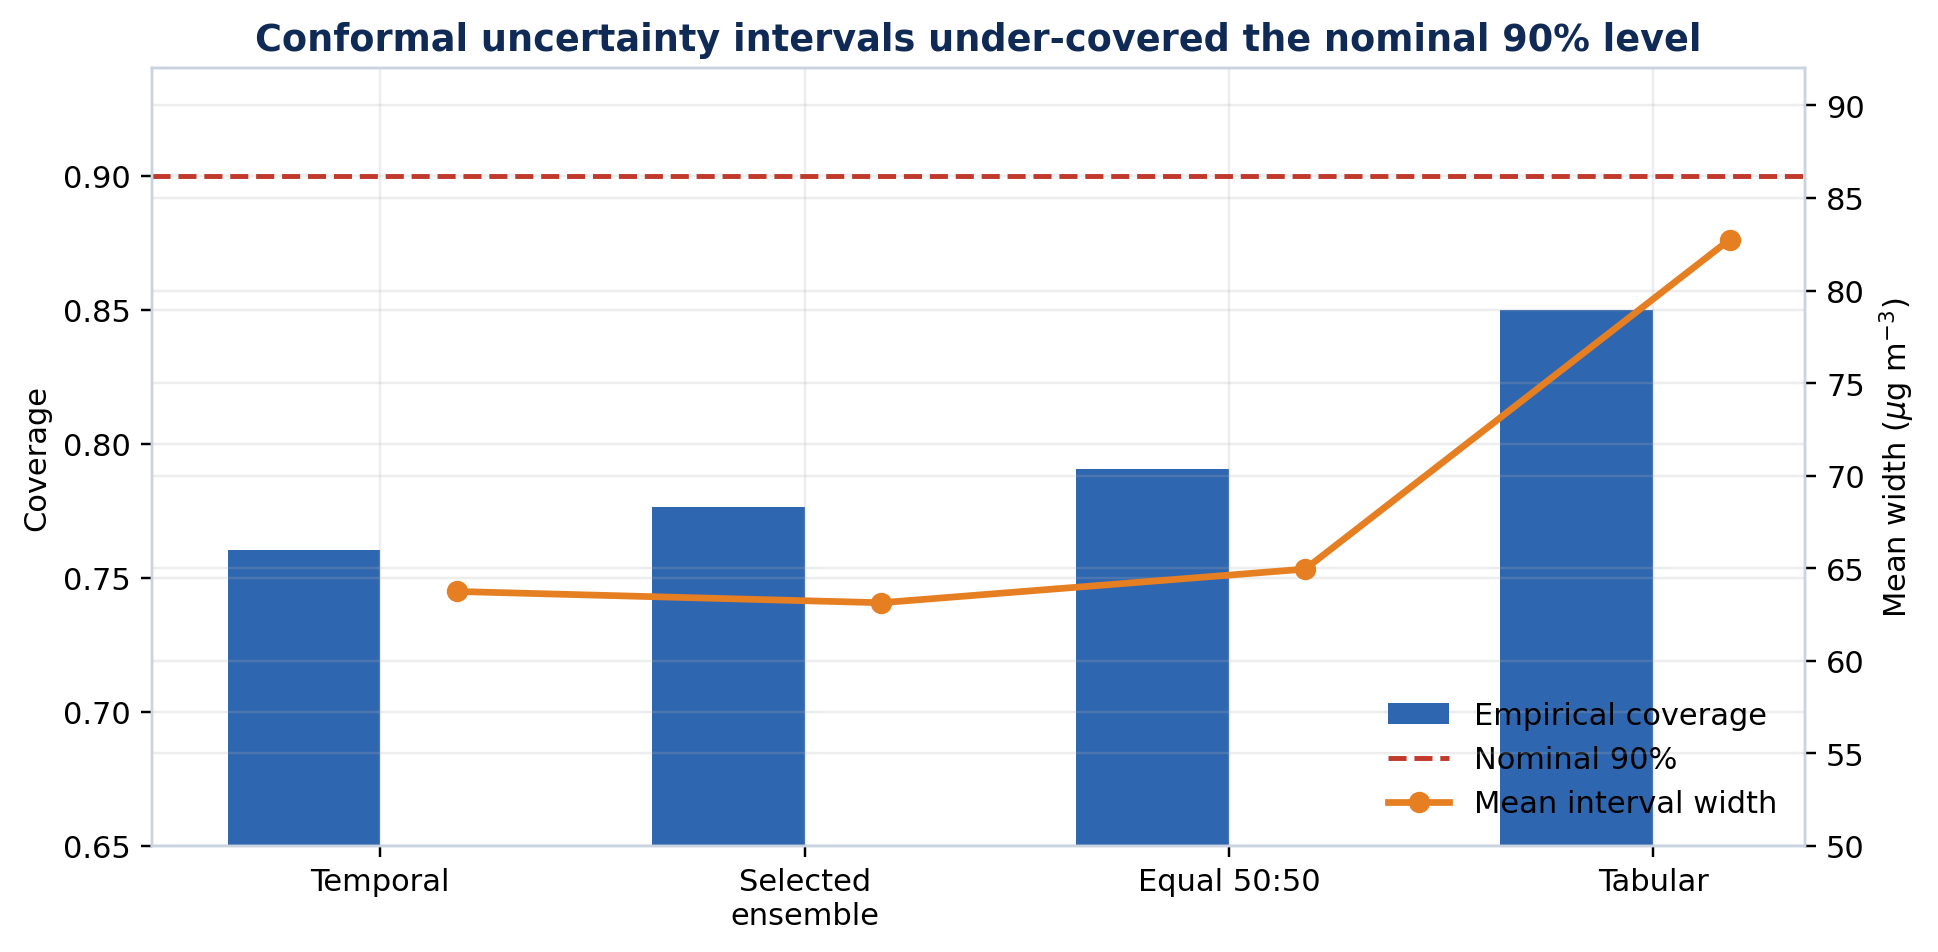
\includegraphics[width=0.84\textwidth]{uncertainty_diagnostics.png}
  \caption{MERRA-2 conformal interval coverage and width. Undercoverage indicates
  residual distribution shift across dates.}
  \label{fig:uncertainty}
\end{figure}
The intervals were therefore informative diagnostics but not yet calibrated
deployment guarantees. Whole-date distribution shift violated the approximate
exchangeability on which simple split-conformal coverage relies.

\chapter{Feature Relevance and Diagnostics}

\section{Correlation and confounding}
Feature relevance was assessed using three complementary views:
\begin{enumerate}
  \item global Pearson and Spearman correlations;
  \item correlations after centring within each date; and
  \item held-out-date permutation importance.
\end{enumerate}
The distinction between global and within-date association was essential.
Total vehicle count, for example, had global Spearman correlation of
approximately -0.179 but within-date correlation of approximately +0.180.
This sign reversal is consistent with route and date confounding. Car-heavy
segments may have occurred on dates or routes with lower regional background;
it does not imply that cars reduce particulate matter.

Repeated preliminary signals included:
\begin{itemize}
  \item \textbf{AlphaEarth:} A52, A51, A06, A49, A10, A14, A36, A39 and A46;
  \item \textbf{road:} lens-6 Laplacian texture, edge density, glare, maximum
        road area, gray/dry ratio and saturation;
  \item \textbf{traffic:} lens-2 vehicle box area, lens-6 total vehicles,
        auto-rickshaws, buses, heavy vehicles and exhaust/resuspension proxies;
  \item \textbf{OSM:} commercial count, service roads, bus stops, total road
        length and hospital count.
\end{itemize}
Only AlphaEarth A36 was selected in every nested feature-selection fold. Hard
top-30 selection still reduced performance, so the final model retained the
broader feature representation.

\section{Spatial variogram}
An empirical variogram was computed from all \num{6873} \pmtwo\ observations using
Haversine distance between latitude/longitude pairs. Within-date semivariance
in the first 0--0.5 km bin was 924.13. The analysis showed spatial structure,
but repeated routes and temporal evolution were confounded with distance.
Consequently, the variogram was treated as a descriptive diagnostic rather than
a fitted stationary geostatistical model.

\section{Sudden-event audit}
Thirty-five transitions exceeded the 99.5th percentile absolute-change threshold
of 119.74 \ugm. Twelve were immediate reversals. The maximum recorded
\texttt{sPM2} was 1,108.64 \ugm. These events dominate RMSE and may reflect real
plumes, sensor lag, clock misalignment, aggregation effects or spikes. The
project generated exact raw one-second request windows and video timestamps for
all five days so that these cases can be checked against the original stream.

The one-second data should be used for:
\begin{itemize}
  \item sensor-video lag estimation;
  \item alternative aggregation windows;
  \item spike persistence and reversal checks;
  \item response-time modelling; and
  \item synchronisation quality control.
\end{itemize}
It should not be used merely to multiply the number of randomly shuffled,
strongly autocorrelated training rows.

\section{Transfer and calibration experiments}
A TRAQID-style weather/time ExtraTrees model transferred poorly to MUMMA:
zero-shot MAE 40.62, RMSE 60.23, \Rtwo\ -0.332 and Spearman 0.195 over all
\num{6873} rows. Retraining the same family improved random interpolation but
not unseen-date performance. Nested five-date raw weather/time ExtraTrees
obtained RMSE 61.44 and \Rtwo\ -0.386; affine calibration worsened it. This
demonstrated that simple linear recalibration cannot repair a change in the
conditional relationship between context and roadside concentration.

\chapter{Particle Regimes and Source Proxies}

\section{Why the terminology changed}
The available sensor table contained cumulative PM mass channels and OPC-like
number channels, not chemically speciated reference contributions. Chemical
source apportionment normally requires source-discriminating tracers, validated
source profiles or differential particle bins. The project therefore adopted
three increasingly cautious labels:
\begin{enumerate}
  \item \emph{latent source-proxy components} for NMF factors;
  \item \emph{assumption-conditioned source scenarios} for profile-based NNLS;
        and
  \item \emph{directly derived particle-size regimes} for algebraic mass/number
        targets.
\end{enumerate}

\section{Train-partition NMF components}
Non-negative matrix factorisation was applied to:
\texttt{sPM1}, \texttt{sPM2}, \texttt{sPM4}, \texttt{sPM10},
\texttt{sNPMp5}, \texttt{sNPM1}, \texttt{sNPM2}, \texttt{sNPM4},
\texttt{sNPM10} and \texttt{sTPS}. NMF was fitted on the training partition
only. Four latent components reconstructed the normalised particle table with
RMSE 0.000649 and exact numerical mass closure.

An ExtraTrees context model predicted component fractions from 127
sensor-plus-visual non-PM variables. On the random test split, component \Rtwo\
values were 0.508, -3.757, -2.382 and 0.604, with macro fraction MAE 0.0897.
The factors are mathematical co-variation patterns. The labels
``component 1'' through ``component 4'' deliberately avoid unsupported names
such as exhaust or road dust.

\section{Assumed-profile scenarios}
Four illustrative profiles represented vehicle exhaust, road dust, secondary
background and unresolved material. Monte Carlo NNLS with 200 draws propagated
profile uncertainty. The assumed profile matrix had condition number 126.9 and
maximum pairwise cosine similarity 0.970. The median solution assigned 100\%
to the vehicle scenario, with nearly all other fractions zero.

This apparently decisive solution was actually an identifiability failure. The
profiles were too similar relative to the available measurements; the solver
selected a boundary solution. The experiment was therefore retained as an
assumption-sensitivity demonstration and explicitly rejected as measured source
apportionment.

\section{Derived particle-size regimes}
Mass increments and number proxies were used to derive four PM$_{10}$ mass
fractions, an effective diameter, a provisional effective-density proxy and a
number proxy. In a random row split, the four mass fractions achieved \Rtwo\
near 0.744, effective diameter 0.648, density proxy 0.544 and total-number proxy
0.844. Held-out-date performance collapsed. On the February 1 stress test,
representative \Rtwo\ values were approximately -72 for a mass fraction, -6.16
for effective diameter, -2.13 for density and -5.12 for number.

\begin{figure}[H]
  \centering
  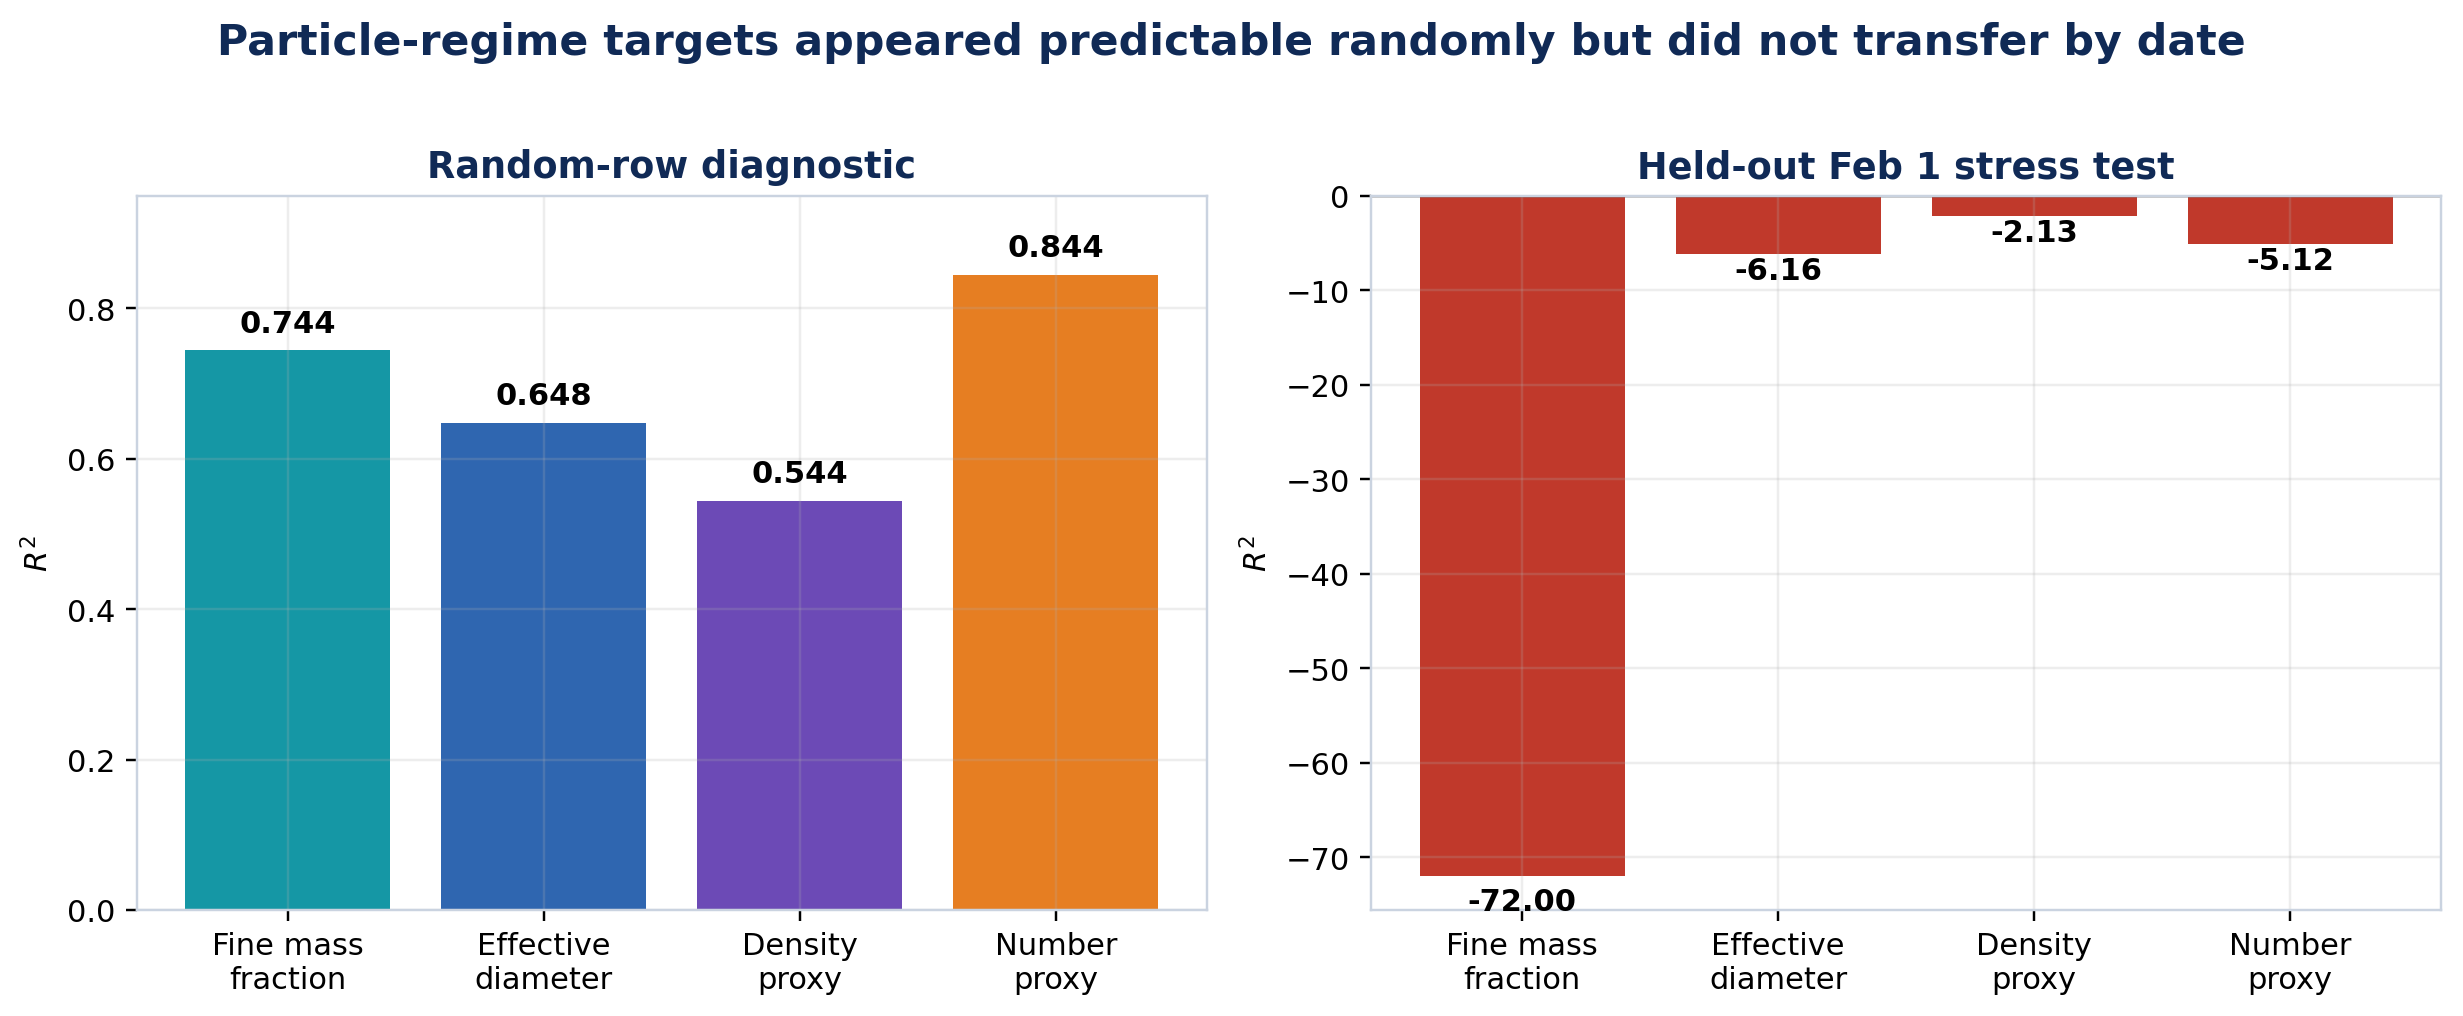
\includegraphics[width=0.94\textwidth]{particle_regime_results.png}
  \caption{Random and held-out-date particle-regime results. The large gap
  mirrors the validation problem found in \pmtwo\ prediction.}
  \label{fig:particle}
\end{figure}

\section{Requirements for credible source attribution}
Future chemical attribution requires:
\begin{itemize}
  \item raw differential OPC bins with confirmed units and cut diameters;
  \item independent chemical/speciation measurements such as FTIR or elemental
        tracers;
  \item source reference samples or defensible literature profiles;
  \item uncertainty-aware receptor modelling and identifiability diagnostics;
        and
  \item held-out event/date validation.
\end{itemize}
Until these data exist, traffic, road, OSM and image variables can support
predictive association and local-increment modelling, not chemical source
percentages.

\chapter{Two-Month Internship Chronology}

\begin{figure}[H]
  \centering
  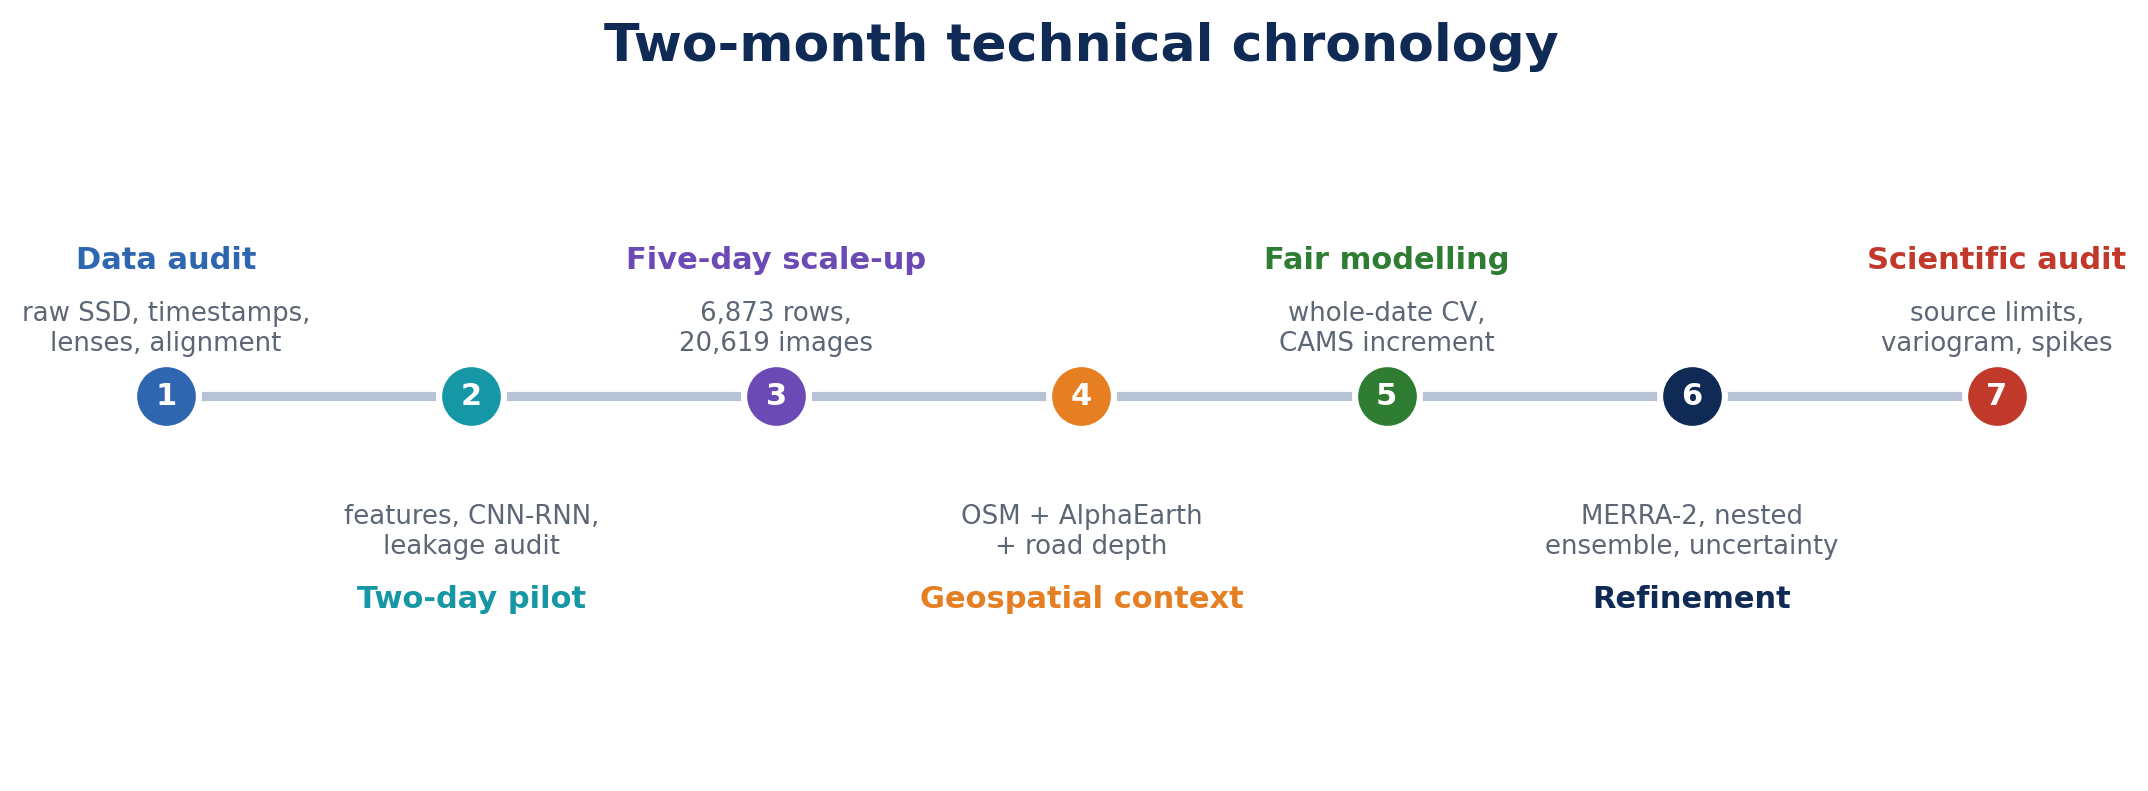
\includegraphics[width=\textwidth]{internship_chronology.png}
  \caption{Technical progression of the internship. The stages were iterative;
  later validation findings caused earlier claims to be revised.}
  \label{fig:chronology}
\end{figure}

\section{Phase 1: repository and data audit}
The first phase identified existing TRAQID code, raw MUMMA folder structure,
sensor columns, camera lenses, timestamp conventions and storage constraints.
The ingestion tools were designed to read the mounted SSD without modifying
it. Configuration files, manifests and artifact directories were used instead
of manual file copying.

\section{Phase 2: two-day pilot}
The two-day pilot validated frame extraction, preprocessing, YOLO traffic,
SegFormer road features and ResNet50 sequence training. Initial random T=3,
T=7 and T=9 experiments revealed strong scores. The overlap audit then showed
that these scores were heavily contaminated, motivating a separate fair
protocol.

\section{Phase 3: five-day scale-up}
Data for February 2, 4 and 5 were ingested, extracted and preprocessed, then
combined with February 1 and 3. The identity audit confirmed \num{6873} sensor
samples and \num{20619} successful frames. YOLO and road features were recomputed
for the complete dataset.

\section{Phase 4: geospatial and atmospheric context}
OSM extraction was initially slow because public Overpass queries timed out.
A tiled persistent cache and local radius filtering reduced repeated network
work; the final run reused 41 of 42 tiles. AlphaEarth embeddings were obtained
for all samples. CAMS, ERA5 and MERRA-2 atmospheric products were aligned by
time and representative location.

\section{Phase 5: architecture ladder and fair validation}
ResNet50, ConvNeXt-tiny, MobileNetV2, GRU, LSTM, multiple views, robust targets,
tabular models and residual correction were compared. Whole-date evaluation
showed that none of the direct image variants solved daily distribution shift.
The project moved from direct \pmtwo\ prediction to background-plus-local-increment
modelling and then to a nested temporal-tabular ensemble.

\section{Phase 6: refinement, uncertainty and alternative architecture}
MERRA-2 replaced CAMS as the strongest tested background. Compact feature
budgets, multi-source background combinations, validation-selected and fixed
ensemble weights, conformal intervals and target-fitted atmospheric calibration
were evaluated. The professor-proposed early image-atmosphere fusion architecture
was implemented on both MUMMA and TRAQID and found not to outperform
atmosphere-only.

\section{Phase 7: scientific audit and communication}
The final phase consolidated model registries, architecture diagrams, full
presentation documentation and careful claims. Feature correlations were
reinterpreted in light of date confounding. Variogram and sudden-event analyses
were added. Source-apportionment language was revised to reflect the limitations
of the measurements.

\chapter{Discussion}

\section{What worked}
The strongest methodological improvement was not a larger CNN. It was the
explicit separation of regional background from local roadside increment.
Direct image models had to infer both broad daily pollution level and local
variation from a short visual sequence. External atmosphere supplied the first
part, allowing visual and geospatial variables to focus on the second.

Temporal and tabular branches proved complementary. The GRU captured persistence
and scene evolution. The tabular branch exposed traffic counts, road state and
slow land-use context. Averaging their errors reduced pooled RMSE. MERRA-2 was
more helpful than CAMS in these five dates, but this is an empirical dataset
result rather than a universal ranking of the products.

\section{What did not work}
Important negative results were:
\begin{itemize}
  \item longer overlapping windows inflated some random scores but did not
        improve whole-date generalisation;
  \item multi-lens concatenation did not consistently beat lens 6 fairly;
  \item ConvNeXt, LSTM, MobileNet and robust loss/date balancing did not resolve
        date shift;
  \item road depth/metric area was noisy and generally harmful;
  \item OSM provided small standalone gains but did not improve the selected
        nested CAMS ensemble;
  \item top-30 feature selection was worse than all 192 visual/geospatial
        features;
  \item affine or target-fitted atmospheric calibration did not repair the
        generalisation problem;
  \item early image-atmosphere fusion added almost nothing over atmosphere-only;
        and
  \item source-proxy patterns did not generalise by date.
\end{itemize}
Retaining these results prevents repeated work and supports a more honest final
claim.

\section{Why the final features are not redundant}
The professor's question about redundancy is scientifically important. If road
dust and vehicle emissions are already in the atmosphere, why include road and
vehicle features? The answer is one of measurement scale and observability:
\begin{enumerate}
  \item the external background represents a coarse regional state, not the
        exact roadside plume;
  \item raw images are high-dimensional and ambiguous; an ImageNet embedding is
        not guaranteed to preserve exact vehicle counts or road-surface cues;
  \item YOLO and road features provide stable, explicit summaries suited to a
        small-data tree model;
  \item OSM and AlphaEarth describe persistent context not fully visible in one
        frame; and
  \item the model does not add ``vehicle PM'' and ``road PM'' as measured
        masses. It uses these variables jointly to predict one local residual.
\end{enumerate}
Thus, the features are different noisy views of the conditions governing the
local increment. Their usefulness must still be established by ablation and
held-out data, not by physical storytelling alone.

\section{Interpretation of current performance}
The validation-selected MERRA-2 ensemble explains 53.8\% of pooled variance and
reduces RMSE to 35.69 \ugm. This is a meaningful improvement over direct fair
models, but it is not a 70--80\% generalisation result. The negative mean
date-specific \Rtwo\ shows that the model is better at capturing differences
between days than fine fluctuations within every day.

The fixed 50:50 diagnostic has higher pooled \Rtwo\ (0.566), but adopting it
after inspecting outer-test performance would constitute test-set model
selection. The scientifically defensible primary result remains the
validation-selected row. A future-date experiment can fairly compare
pre-specified selected and 50:50 policies if both are frozen in advance.

\section{Threats to validity}
\begin{itemize}
  \item Only five MUMMA dates were available, with unequal routes and sample
        counts.
  \item The same dates informed repeated exploratory decisions.
  \item External backgrounds are model/reanalysis fields, not independent
        roadside measurements.
  \item Extreme sensor values may include real events and timing/quality
        artefacts.
  \item Image and sensor clocks may have residual lag.
  \item AlphaEarth dimensions are latent and OSM completeness is location
        dependent.
  \item Pooled metrics can conceal poor within-date performance.
  \item Simple conformal intervals under-covered under date shift.
\end{itemize}

\chapter{Conclusions and Future Work}

\section{Conclusions}
This internship transformed a visually impressive but overlap-sensitive
image-sequence benchmark into a multimodal, leakage-audited research pipeline.
The work showed that:
\begin{enumerate}
  \item random-window scores as high as 0.95--0.97 can be reproduced but are not
        evidence of unseen-date generalisation;
  \item direct CNN-RNN and tabular models struggle under whole-date shift;
  \item separating external atmospheric background from local roadside
        increment materially improves fair pooled performance;
  \item MERRA-2 was the strongest tested background on five-day MUMMA;
  \item temporal and tabular local branches provide complementary predictions;
  \item current pooled performance remains accompanied by negative mean
        per-date \Rtwo; and
  \item chemical source attribution is not supported by the current sensor
        channels.
\end{enumerate}

\section{Frozen candidate for future-date confirmation}
The recommended confirmatory pipeline is:
\begin{enumerate}
  \item align and preprocess lens-6 frames at the sensor timestamps;
  \item encode frames with frozen ResNet50 and build T=7 sequences within
        \texttt{run\_id};
  \item retrieve MERRA-2 background without fitting it to roadside targets;
  \item train the GRU on the local increment;
  \item cross-fit a sensor/YOLO/road Random Forest residual correction by run;
  \item train a YOLO/road/OSM/AlphaEarth ExtraTrees local branch;
  \item choose the convex temporal/tabular weight on validation predictions
        only;
  \item calibrate an uncertainty interval on validation residuals;
  \item freeze preprocessing, features, architecture, hyperparameters and
        weights; and
  \item evaluate once on untouched future dates.
\end{enumerate}

\section{Priority future experiments}
\begin{enumerate}
  \item Collect new dates spanning different routes, weather, traffic and
        pollution regimes.
  \item Obtain raw one-second streams and estimate sensor-video lag before
        retraining.
  \item Add independent regulatory or local background monitors where possible
        to evaluate and bias-correct atmospheric products without using the
        roadside test target.
  \item Use group-aware domain adaptation only within nested training data.
  \item Model extreme events separately or use mixture/quantile objectives.
  \item Recalibrate uncertainty using leave-one-date-out or weighted conformal
        methods designed for distribution shift.
  \item Confirm OPC units and obtain differential bins plus chemical reference
        measurements before restarting source attribution.
\end{enumerate}

\section{Final scientific statement}
The project has identified a promising and reproducible approach, not a
deployment-ready universal predictor. Its most important outcome is the
combination of engineering completeness and scientific restraint: a full
multimodal pipeline, an improved background-aware model, explicit leakage
audits, transparent negative results and a clear decisive next experiment.

\appendix

\chapter{Reproducibility and Artifact Index}

\section{Canonical data products}
\begin{longtable}{p{0.31\textwidth}p{0.62\textwidth}}
  \toprule
  Artifact & Repository path\\
  \midrule
  \endfirsthead
  \toprule
  Artifact & Repository path\\
  \midrule
  \endhead
  Five-day sensor table &
  \path{artifacts/runs/mumma_5day_combined_lenses_1_2_6_v1/sensor_10s.csv}\\
  Five-day frame manifest &
  \path{artifacts/runs/mumma_5day_combined_lenses_1_2_6_v1/manifests/preprocessed_frames.csv}\\
  YOLO frame features &
  \path{artifacts/runs/mumma_5day_visual_features_v1/yolo_frame_features.csv}\\
  YOLO objects &
  \path{artifacts/runs/mumma_5day_visual_features_v1/yolo_objects.csv}\\
  Road features &
  \path{artifacts/runs/mumma_5day_visual_features_v1/road_features_lenses_1_6.csv}\\
  OSM 250 m context &
  \path{artifacts/runs/mumma_5day_geospatial_corridor_v1/osm_250m.csv}\\
  AlphaEarth embeddings &
  \path{artifacts/runs/mumma_5day_geospatial_alphaearth_v1/alphaearth_2025_point.csv}\\
  Atmospheric background &
  \path{artifacts/runs/mumma_5day_atmospheric_background_v1/background_hourly.csv}\\
  Canonical non-PM modelling table &
  \path{artifacts/runs/mumma_5day_complete_nonpm_models_v1/modeling_table.csv}\\
  Feature groups &
  \path{artifacts/runs/mumma_5day_complete_nonpm_models_v1/feature_groups.json}\\
  \bottomrule
\end{longtable}

\section{Principal model artifacts}
\begin{longtable}{p{0.34\textwidth}p{0.59\textwidth}}
  \toprule
  Experiment & Repository path\\
  \midrule
  \endfirsthead
  \toprule
  Experiment & Repository path\\
  \midrule
  \endhead
  Five-day fair image ladder &
  \path{artifacts/runs/mumma_5day_image_ladder_T7_gru_v1}\\
  Direct complete tabular benchmark &
  \path{artifacts/runs/mumma_5day_complete_nonpm_models_v1}\\
  CAMS local increment &
  \path{artifacts/runs/mumma_5day_background_local_increment_osm_alphaearth_v1}\\
  CAMS nested ensemble &
  \path{artifacts/runs/mumma_5day_nested_background_ensemble_fair_v1}\\
  CAMS nested ensemble with OSM &
  \path{artifacts/runs/mumma_5day_nested_background_ensemble_osm_fair_v1}\\
  MERRA-2 local increment &
  \path{artifacts/runs/mumma_5day_merra2_local_osm_alphaearth_fair_v1}\\
  MERRA-2 nested ensemble &
  \path{artifacts/runs/mumma_5day_nested_merra2_ensemble_osm_fair_v1}\\
  MERRA-2 ensemble + uncertainty &
  \path{artifacts/runs/mumma_5day_nested_merra2_ensemble_osm_uncertainty_fair_v1}\\
  Architecture-2 MUMMA &
  \path{artifacts/runs/mumma_5day_architecture2_stage1_fusion_fair_v1}\\
  Architecture-2 TRAQID &
  \path{artifacts/runs/traqid_architecture2_stage1_fusion_fair_v1}\\
  TRAQID matched random backgrounds &
  \path{artifacts/runs/traqid_T7_background_random_comparison_v1}\\
  TRAQID nested backgrounds &
  \path{artifacts/runs/traqid_T7_nested_background_ensemble_fair_v1}\\
  \bottomrule
\end{longtable}

\section{Project documentation}
\begin{itemize}
  \item \path{docs/pm25_experiment_consolidation.md}: audited PM modelling story.
  \item \path{docs/model_architecture_catalog.md}: architecture-by-architecture
        code and status catalogue.
  \item \path{docs/pm25_model_registry.csv}: exact PM result index.
  \item \path{docs/model_architecture_registry.csv}: architecture registry.
  \item \path{docs/experiment_registry.csv}: run-level experiment inventory.
  \item \path{docs/complete_project_export_for_presentation.md}: broad project
        export used for presentation development.
  \item \path{docs/data_lineage.md}: dataset lineage and processing paths.
\end{itemize}

\chapter{Detailed Feature Dictionary}

\section{YOLO feature semantics}
\begin{longtable}{p{0.22\textwidth}p{0.31\textwidth}p{0.39\textwidth}}
  \toprule
  Category & Representative variables & Interpretation\\
  \midrule
  \endfirsthead
  \toprule
  Category & Representative variables & Interpretation\\
  \midrule
  \endhead
  Vehicle totals & total, motor and heavy vehicle counts & Instantaneous traffic
  activity and fleet composition.\\
  Classes & car, motorcycle, auto-rickshaw, bus, truck, bicycle, fallback &
  Explicit mix of visually detected road users.\\
  Confidence & average and maximum confidence & Detection certainty and scene
  difficulty; not an emission variable.\\
  Box geometry & mean/max box area and occupancy & Proxy for proximity and visual
  scene occupancy.\\
  Exhaust proxy & class-weighted initial exhaust score & Heuristic source
  opportunity; not measured exhaust mass.\\
  Resuspension proxy & class/size-weighted road activity score & Heuristic
  opportunity for mechanically generated dust.\\
  Per-lens variants & lens 1, 2 and 6 copies & Preserves view-specific traffic
  information rather than averaging all cameras blindly.\\
  Availability & \texttt{yolo\_lens\_count} & Quality-control indicator for
  available views.\\
  \bottomrule
\end{longtable}

\section{Road feature semantics}
\begin{longtable}{p{0.27\textwidth}p{0.58\textwidth}}
  \toprule
  Variable & Interpretation\\
  \midrule
  \endfirsthead
  \toprule
  Variable & Interpretation\\
  \midrule
  \endhead
  Road area ratio & Fraction of the image classified as road.\\
  Mean brightness & Illumination of the road mask.\\
  Mean saturation & Colour intensity, potentially affected by surface and
  lighting.\\
  Contrast standard deviation & Variation in road appearance.\\
  Shadow/glare ratios & Illumination artefacts and surface reflectance.\\
  Brown-pixel ratio & Heuristic colour proxy for dusty/bare-looking road.\\
  Gray/dry-pixel ratio & Heuristic dry pavement appearance.\\
  Edge density & Fine spatial structure and markings/texture.\\
  Laplacian standard deviation & High-frequency texture/sharpness.\\
  Haze-flatness proxy & Low-contrast appearance proxy; not direct aerosol optical
  depth.\\
  \bottomrule
\end{longtable}

\section{OSM feature semantics}
\begin{longtable}{p{0.30\textwidth}p{0.55\textwidth}}
  \toprule
  Feature group & Context represented\\
  \midrule
  \endfirsthead
  \toprule
  Feature group & Context represented\\
  \midrule
  \endhead
  Fuel stations, bus stops, parking & Traffic generation, stopping and idling
  opportunities.\\
  Restaurants, marketplaces, commercial, retail & Human activity, delivery,
  parking and congestion context.\\
  Construction, industrial, factory, warehouse & Heavy-vehicle, loading and
  dust-source opportunity.\\
  Schools, hospitals, parks & Land-use and activity context.\\
  Road count and total length & Local network density.\\
  Motorway through service/living street counts & Road hierarchy and likely
  traffic function.\\
  \bottomrule
\end{longtable}

\chapter{Model and Experiment Status}

\begin{longtable}{p{0.30\textwidth}p{0.20\textwidth}p{0.40\textwidth}}
  \toprule
  Experiment family & Status & Main conclusion\\
  \midrule
  \endfirsthead
  \toprule
  Experiment family & Status & Main conclusion\\
  \midrule
  \endhead
  TRAQID OOF clipped residual & Complete, random diagnostic & Highest historical
  \Rtwo\ 0.966; overlap-contaminated.\\
  MUMMA two-day sequence ladder & Complete, exploratory & Longer T improved
  random score and leakage simultaneously.\\
  Five-day frozen-CNN ladder & Complete, fair & Backbone changes did not solve
  date shift.\\
  Five-day LSTM random run & Incomplete & Sequences/audit exist; no final
  training metrics found.\\
  Five-day direct tabular & Complete & Random interpolation strong; fair
  visual/geospatial \Rtwo\ about 0.16.\\
  Depth road area & Complete, rejected feature & Provisional values were heavily
  flagged and generally harmful.\\
  OSM & Complete & Useful context; small matched gain; no full-ensemble gain.\\
  AlphaEarth & Complete & Distributed latent signal; top-30 selection harmful.\\
  CAMS local increment & Complete & Major fair improvement to pooled \Rtwo\
  about 0.425--0.457.\\
  MERRA-2 local increment & Complete & Strongest tested five-day background;
  pooled \Rtwo\ 0.550 standalone.\\
  MERRA-2 nested ensemble & Complete, exploratory candidate & Selected pooled
  \Rtwo\ 0.538; equal-weight diagnostic 0.566.\\
  Conformal uncertainty & Complete, diagnostic & Intervals under-covered under
  date shift.\\
  Architecture 2 early fusion & Complete on both datasets & Did not beat
  atmosphere-only.\\
  NMF source proxies & Complete, exploratory & Some random component
  predictability; no chemical identities.\\
  Assumed source scenarios & Complete, rejected inference & Degenerate,
  ill-conditioned solution.\\
  Particle regimes & Complete, exploratory & Strong random results; poor
  held-out-date transfer.\\
  Variogram and sudden events & Complete, diagnostic & Spatial/time confounding
  and extreme-event validation needs identified.\\
  \bottomrule
\end{longtable}

\chapter{Build Instructions}
The report source and generated figures are self-contained inside
\path{docs/internship_report}. To rebuild:
\begin{verbatim}
cd docs/internship_report
python3 generate_figures.py
latexmk -pdf -interaction=nonstopmode internship_report.tex
\end{verbatim}
If \texttt{latexmk} is unavailable, two passes of \texttt{pdflatex} are
sufficient for the table of contents and references:
\begin{verbatim}
pdflatex internship_report.tex
pdflatex internship_report.tex
\end{verbatim}
The final identity fields are defined at the top of the \LaTeX{} source and can
be edited without searching through the document.

\begin{thebibliography}{99}

\bibitem{he2016resnet}
K. He, X. Zhang, S. Ren and J. Sun,
``Deep Residual Learning for Image Recognition,''
\emph{Proceedings of the IEEE Conference on Computer Vision and Pattern
Recognition}, 2016.

\bibitem{cho2014gru}
K. Cho et al.,
``Learning Phrase Representations using RNN Encoder-Decoder for Statistical
Machine Translation,''
\emph{Proceedings of EMNLP}, 2014.

\bibitem{hochreiter1997lstm}
S. Hochreiter and J. Schmidhuber,
``Long Short-Term Memory,''
\emph{Neural Computation}, vol. 9, no. 8, pp. 1735--1780, 1997.

\bibitem{breiman2001rf}
L. Breiman,
``Random Forests,''
\emph{Machine Learning}, vol. 45, pp. 5--32, 2001.

\bibitem{geurts2006extratrees}
P. Geurts, D. Ernst and L. Wehenkel,
``Extremely Randomized Trees,''
\emph{Machine Learning}, vol. 63, pp. 3--42, 2006.

\bibitem{xie2021segformer}
E. Xie et al.,
``SegFormer: Simple and Efficient Design for Semantic Segmentation with
Transformers,''
\emph{Advances in Neural Information Processing Systems}, 2021.

\bibitem{gelaro2017merra2}
R. Gelaro et al.,
``The Modern-Era Retrospective Analysis for Research and Applications, Version
2 (MERRA-2),''
\emph{Journal of Climate}, vol. 30, no. 14, pp. 5419--5454, 2017.

\bibitem{inness2019cams}
A. Inness et al.,
``The CAMS Reanalysis of Atmospheric Composition,''
\emph{Atmospheric Chemistry and Physics}, vol. 19, pp. 3515--3556, 2019.

\bibitem{lee1999nmf}
D. D. Lee and H. S. Seung,
``Learning the Parts of Objects by Non-negative Matrix Factorization,''
\emph{Nature}, vol. 401, pp. 788--791, 1999.

\bibitem{angelopoulos2021conformal}
A. N. Angelopoulos and S. Bates,
``A Gentle Introduction to Conformal Prediction and Distribution-Free
Uncertainty Quantification,''
arXiv:2107.07511, 2021.

\bibitem{osm}
OpenStreetMap contributors,
``OpenStreetMap,''
\url{https://www.openstreetmap.org/}.

\bibitem{pytorch}
A. Paszke et al.,
``PyTorch: An Imperative Style, High-Performance Deep Learning Library,''
\emph{Advances in Neural Information Processing Systems}, 2019.

\bibitem{sklearn}
F. Pedregosa et al.,
``Scikit-learn: Machine Learning in Python,''
\emph{Journal of Machine Learning Research}, vol. 12, pp. 2825--2830, 2011.

\end{thebibliography}

\end{document}
